% Development of game engine - core components & functonalities
% development of game using the game engine, including level/scene design (asset creation, scene scripting & interaction, development in general)
% UI / XP Design
% Testing & Debugging (Test cases / scenarios), (Logging, Debugger, Code Analysis), Performance Testing (-> memoization, ...), playtesting?

\chapter{Development \& Implementation}\label{ch:implementation}
In this chapter, the implementation of the game engine including the basic framework, graphic rendering and input handling is described.
The game is implemented by using the game engine framework and its features as a baseline which is extended to the game requirements and goals
defined in the previous chapters.
The game mechanics are developed and programmed in line with the entity-component system approach, as well as the Markov process is explained.
Furthermore, important scene and graphics designs are described as this is integral to understanding the implementation.

\section{General Approach}\label{sec:general-approach}
The game engine is implemented as a separate, independent, enhanceable framework, which may also be used to design other
games.
It provides basic functionality for all features needed to design a game, such as input and system handling, rendering, configuration
classes and managers.
The implementation uses a basic entity-component-system as foundation and enhances this with further features.

\section{Programming Language}\label{sec:programming-language}
The programming language that was chosen for this implementation is \textit{JAVA}.
Java is a high-level, object-oriented programming language that was originally developed by Sun Microsystems (now owned by Oracle Corporation) in the mid-1990s.
It is designed to be portable, meaning that it can be run on a wide variety of platforms, including Windows, macOS,
Linux, and many others, without needing to be recompiled for each platform.
\\
Java is widely used for developing both desktop and web-based applications, as well as mobile applications for Android devices.
It is also used extensively in server-side programming and for building enterprise applications.
\\
One of the key features of Java is its virtual machine (VM), which allows Java programs to be executed on any system that has a compatible JVM installed, regardless of the underlying hardware and operating system.
This makes it possible to write a single Java program that can run on multiple platforms, without needing to be modified for each one.
\\
Java also has a large standard library of classes and functions, which makes it easier to write complex programs without needing to reinvent the wheel.
Additionally, Java is known for its strong emphasis on security, which makes it a popular choice for building applications that need to be highly secure
and resistant to cyber attacks.
\\
Java was chosen because of the wide variety of standard libraries and resources available, the very object-oriented programming approach which enables for
extending and inheriting of classes to adapt objects to the games and game engines needs.
Due to garbage collection, Java enables developing without having to consider memory allocations.
Furthermore, a great benefit of using Java is the multi-platform support due to Java being an interpreted language which works
independent of operating systems or processor architectures~\cite{JAVA}.

\section{Game Engine}\label{sec:game}
The game engine implements a variety of methods and classes which are used for handling the general program execution, independent of the actual game implementation.
In this chapter, these classes will be explained in detail and the general concept of the engine is reviewed.

\subsection{Entity Component System}\label{subsec:entity-component-system-implementation}
The entity component system setup used in this implementation can be approached from a top-down point of view, visualized in figure \ref{fig:ecs}.
A scene is the basic class that contains all information about the currently displayed entities and the handlers and systems to be used
in the background.
There exist multiple scenes of different classes, such as scenes for the game view, menu scenes etc., which can be created by
inheriting the base scene class.
Scenes can be added to the game by using the Scene Manager, which is also used to swap between available scenes.
Each scene contains a list of entities, that could be referred to as a database of all available objects.
Entities represent a combination of different data containers, so-called components, which can be uniquely attached to each entity.
There are some standard entities and components available directly via the engine, however there may be the need for more components and entities while implementing the actual game.
The design approach of this entity component system is similar to the Unity implementation, however some simplifications were made to guarantee ab easily maintainable
and highly customizable game engine, without having to rely on third parties to bring in needed updates.
Furthermore, the simplifications made help with keeping an overview of all features needed and decreases unused features, to keep the engine as non-complex as possible.
\begin{figure}
    \centering
    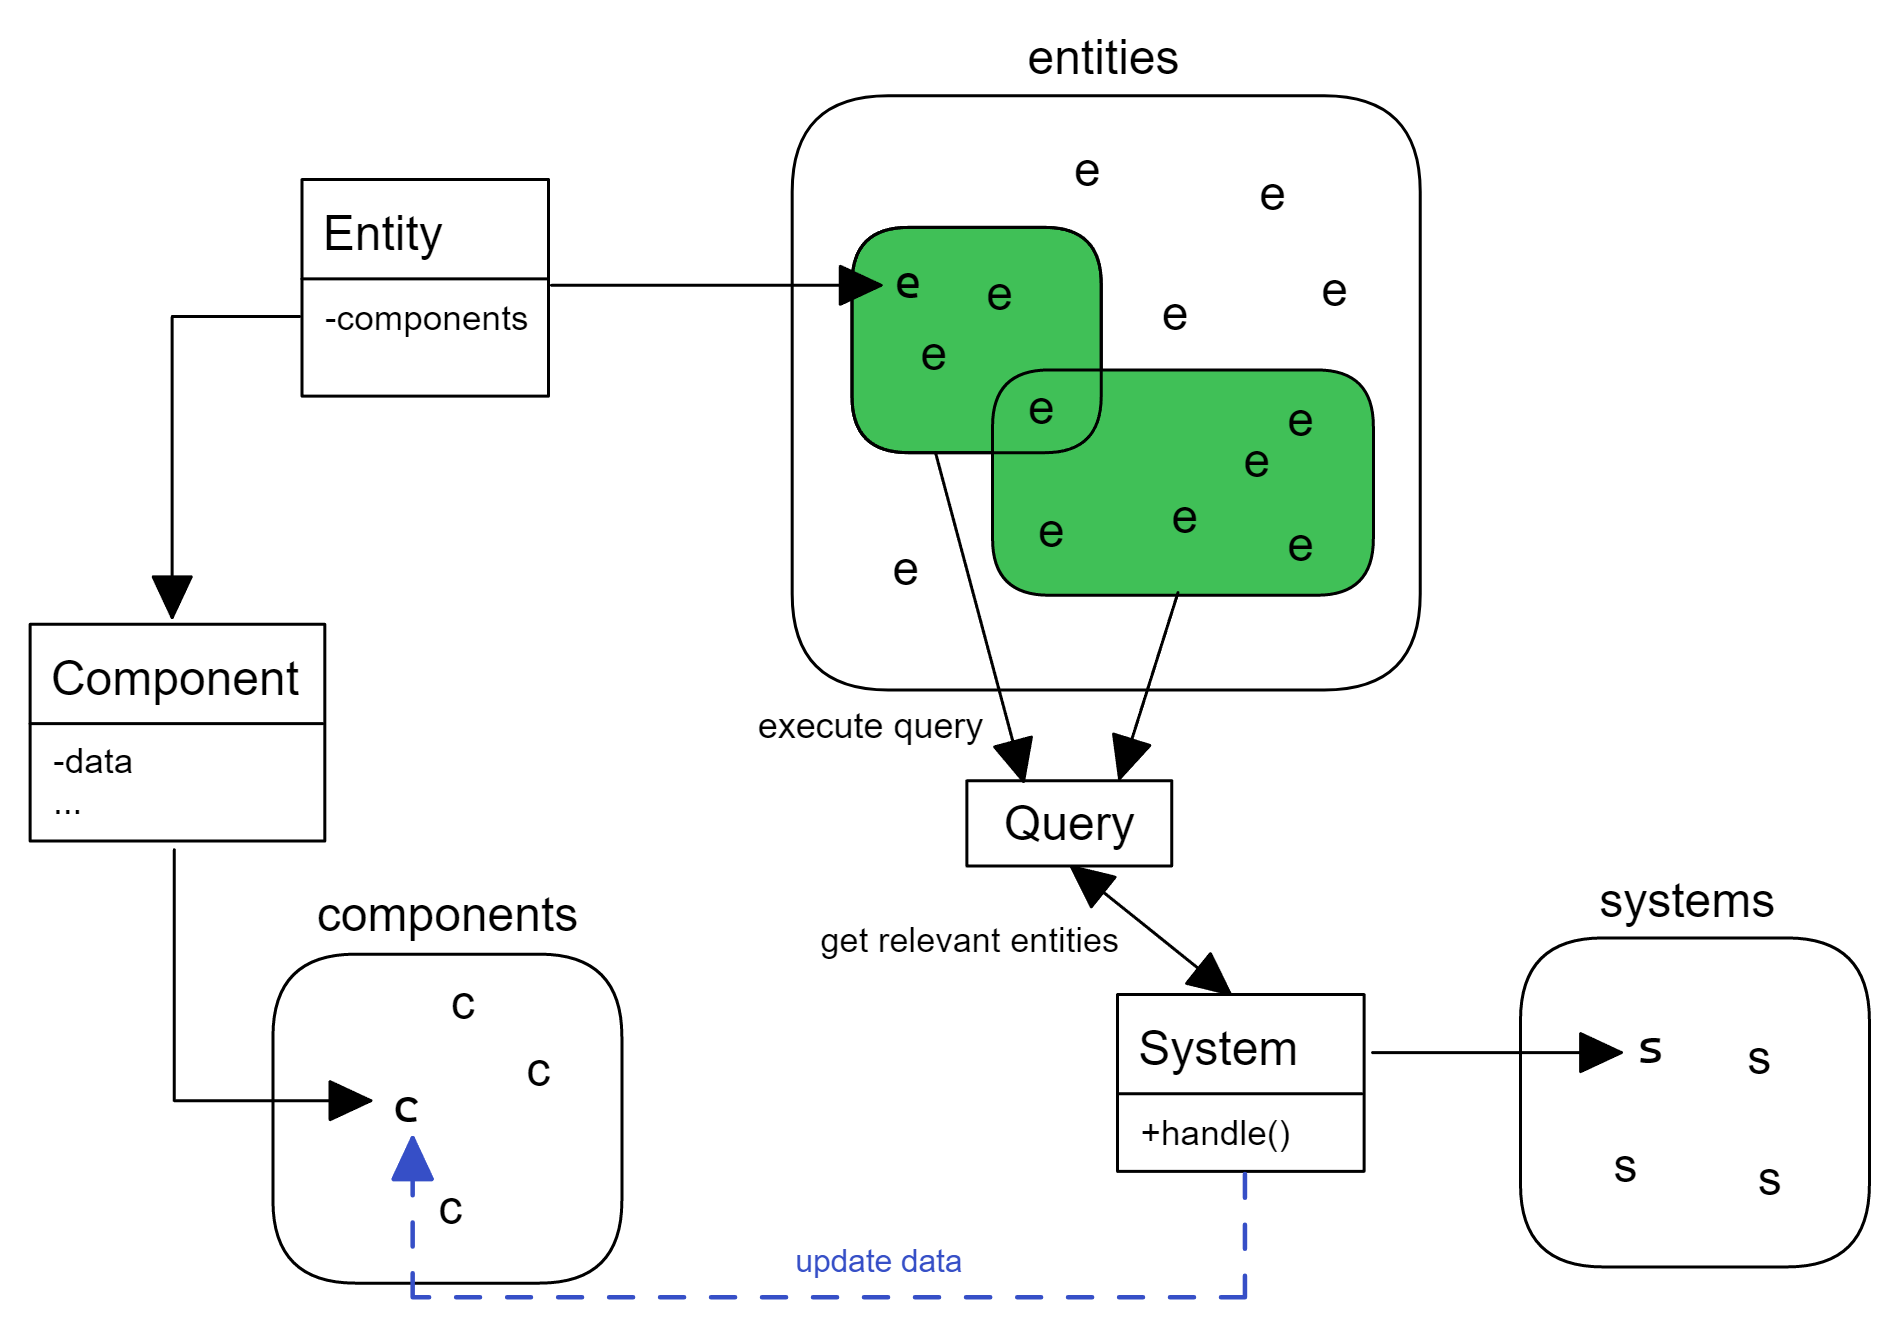
\includegraphics[width=\textwidth]{Pictures/res/implementation/ecs-database}
    \caption{ECS Database}
    \label{fig:ecs}
\end{figure}
\subsubsection{UML Diagram}\label{subsubsec:uml-diagram}
The UML diagram as seen in figure \ref{fig:ecs-block-diagram} shows a simplified structure of the engine implementation, which is going to be used to explain the mechanisms
and the framework of the implementation.
\begin{figure}
    \centering
    
\includegraphics[width=1.0\textwidth]{./Pictures/res/implementation/ecs-uml}
    \caption{Simplified UML diagram of the engine implementation}
    \label{fig:ecs-block-diagram}
\end{figure}

\subsubsection{Entities}\label{subsubsec:entities}
Entities are classes constructed from different, unique components, which could be referred to as containers storing different parameters to
describe the input behaviour of the systems.
Entities can not directly interact with each other, as any modification to data is strictly handled by the game engines' systems and handlers,
however components may contain direct references to other entities if needed.
The Entity class implements functions to add, remove and get Components of a class type.
\\
As there are usually lots of different types of entities in a game which may contain the same components, it makes sense to inherit from the Entity class and
build generic entities which can be reused.
For GUI elements, the game engine already provides some pre-designed entities, such as buttons, text bodies, panels and image entities.
During the implementation, it was chosen to handle GUI elements as entities as well, as the game engine is purely working in 2 dimensions and therefore
rendering methods for the game itself and the GUI do not differ.
This approach was the easy choice, as having a separate class to implement UI elements would most likely end up with a lot of duplicated
code fragments, which are already implemented in the RenderingComponent, as described in the next chapter.
\subsubsection{Components}\label{subsubsec:components}
All entities are built of a subset of the available components, uniquely attached to each.
The components available by default will be explained in detail in the following chapter.

\textbf{Render Component:} \\
The \textit{RenderComponent} class is designed to manage and store a diverse set of graphical objects that are utilized for
rendering various elements within a scene.
These graphical objects are categorized into subclasses, such as text, images, animations, hovering, lines, and shapes.
Each subclass is defined by a set of parameters that dictate its appearance, including aspects like location, bounds, colors,
images or animations, and text content.
\\
To address the need for rendering multiple graphical objects per entity while still adhering to the unique
component-per-entity constraint, the RenderComponent class allows for the addition of each graphical object multiple times.
For example, an image that requires occasional hovering may have one object to render the image itself, and
another object to render the hovering shape.
\\
Furthermore, the RenderComponent class incorporates methods that enable the retrieval of specific lists of
graphical object instances based on their corresponding class.
This functionality resembles the Query implementation found in the entity component system, providing a
streamlined and efficient way to access the desired graphical objects.

\textbf{ColliderComponent:} \\
Similar to the \textit{RenderComponent}, the \textit{ColliderComponent} also stores a list of collision objects, which are described by location and bounds.
Each of these collision objects is checked by the \textit{CollisionDetectionSystem} and handled accordingly, e.g.\
hovering an object at the same location as the collision object.

\textbf{Sound Component:} \\
The \textit{SoundComponent} class can be attached to any entity that needs to have a sound played at times.
It implements methods to set the state of the sound sample to play, pause or stop and contains the actual sound sample to be used by the \textit{SoundEngine}. \\ \\

\textbf{Action Component:} \\
\textit{ActionComponents} are used for storing a mapping of input to action within an entity, e.g.\ clicking a button which opens another scene.
Each \textit{ActionComponent} is processed by the \textit{ActionSystem}.

\textbf{Cursor Component:} \\
The cursor component is a component used for handling game pad inputs and acts as a virtual mouse cursor, which can be moved by using
joysticks of game pads or keyboard buttons.
It simply indicates the position, where new mouse events are generated, when the actual mouse is not used.
\subsubsection{Scene}\label{subsubsec:scene}
A scene is a collection of entities that together form an aspect of the game, e.g.\ a menu or a level.
The \textit{Scene} class is an abstract class implementing methods for adding and removing entities from itself.
\\
To add a scene to the game, a scene object needs to be instantiated and added to the games' \textit{SceneManager}, where all
scenes are stored and the currently active scene can be set.
Generally, all systems access the scene manager to only process the currently active scene, or if needed handle entities in other scenes or add or remove them.
\subsubsection{Systems}\label{subsubsec:systems}
Systems are the third major part of the ECS implementation and handle any modification to the components.
They are used for a variety of different purposes and can be split into multiple sub systems, which each serve their own purpose.
The ECS implementation aims and encourages to split each function or feature into modular systems, which can then be added to the game where they
are handled within the \textit{GameLoop} as explained in section~\ref{subsec:game-loop}.
A variety of systems is already available per default, including rendering, collision and input systems, which will be explained in the following chapters.
\\
Each system queries through the available entities / components and only processes the relevant ones.
The query system is set up as a static class that can be accessed from anywhere.
It implements methods that can be used to search for all entities of a class or entities that have a specified component
attached to it within the currently displayed scene.
The set of entities can be seen as a database that is filtered by the query system to obtain only a subset with the specified component or class type, which may be used
for other systems.
System processing is shown in figure~\ref{fig:ecs-system-processing}.
\begin{figure}
    \centering
    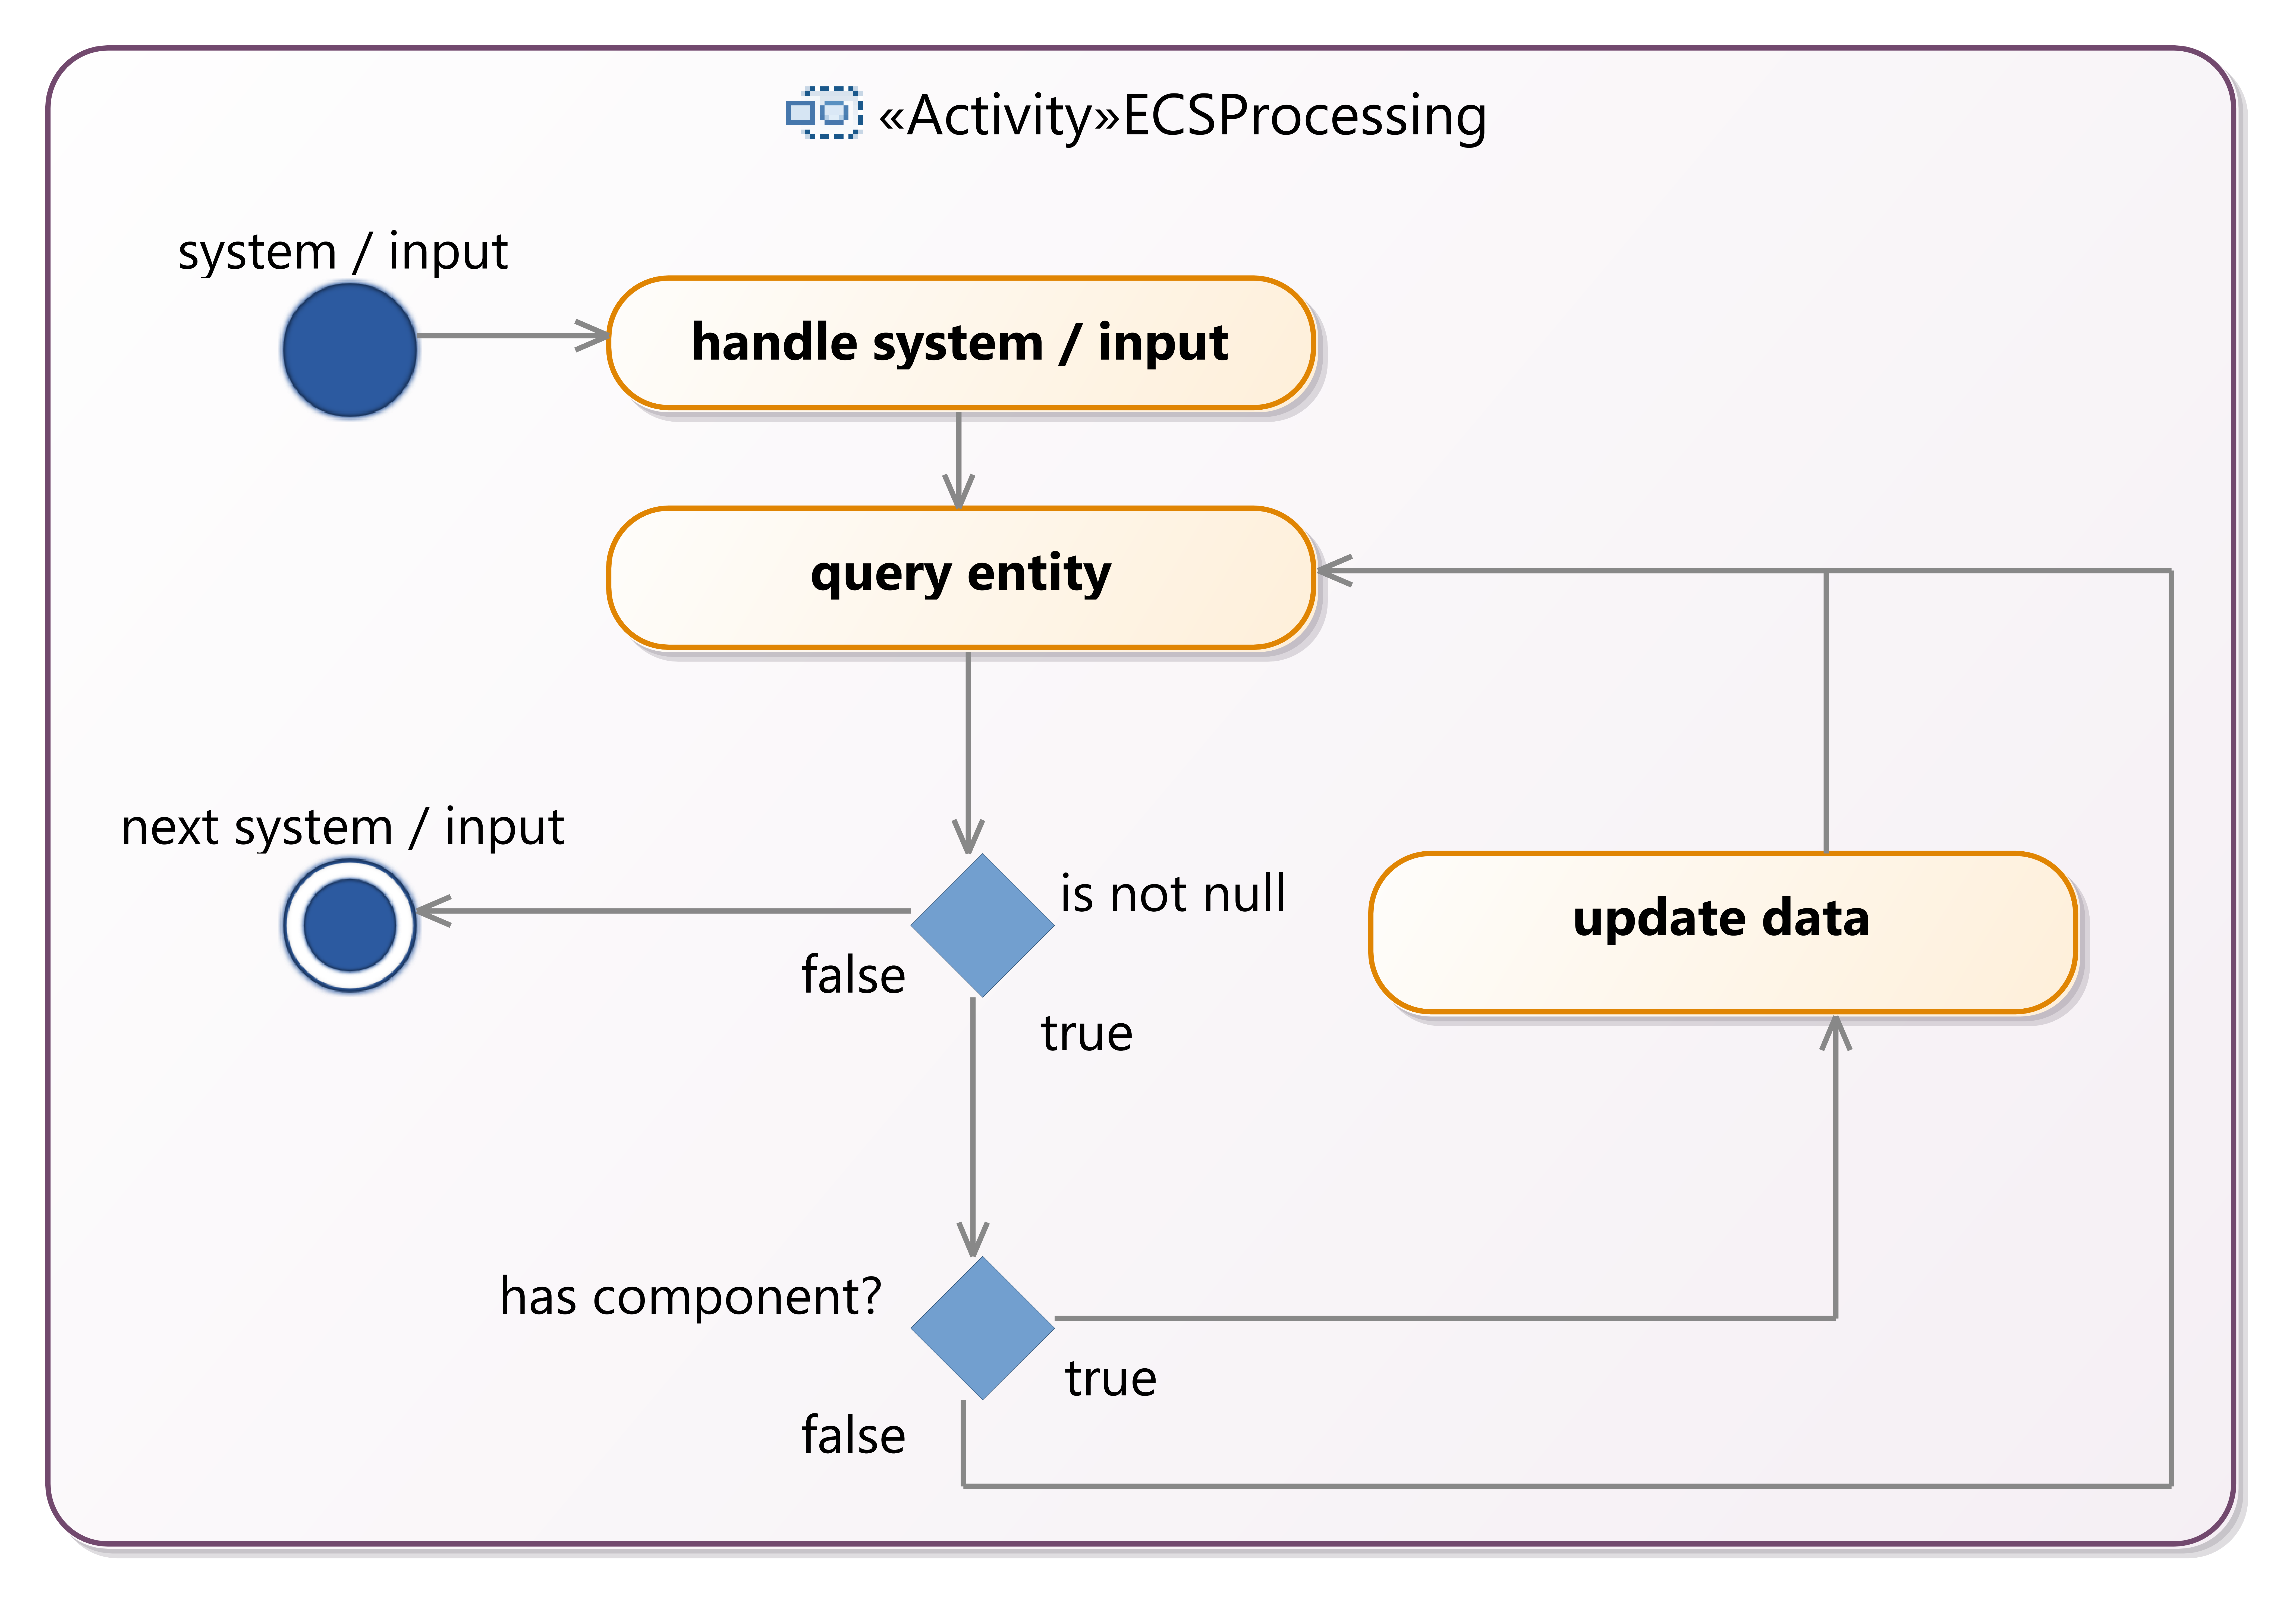
\includegraphics[width=\textwidth]{Pictures/res/implementation/ecs-system-processing}
    \caption{System processing activity diagram}
    \label{fig:ecs-system-processing}
\end{figure}
The systems implemented per default to this game engine are explained with reference to the \textit{GameLoop} implementation
as described in section~\ref{subsec:game-loop}.
\subsection{Game Loop}\label{subsec:game-loop}
The game loop acts as the main thread of the game as soon as initialized and started.
It packs all the different systems and handlers used in the game and executes them in a given order at every time step
$t_{i} = t_{i-1} + \Delta t$, where $\Delta t$ is the execution rate defined for the game.
An exception to this order is the input recording, which is handled in a separate, synchronized thread, as described in chapter~\ref{subsec:input-recording}.
In this implementation, $\Delta t$ is defined as $\Delta t = 1000 / 240 ms = 4.1667 ms$, which equals 240 calculated frames per second that may be shown and rendered
to the screen, if available.
\\ \\
The execution order of the game loop can be seen in figure~\ref{fig:gameloop-process}.
\begin{figure}
    \centering
    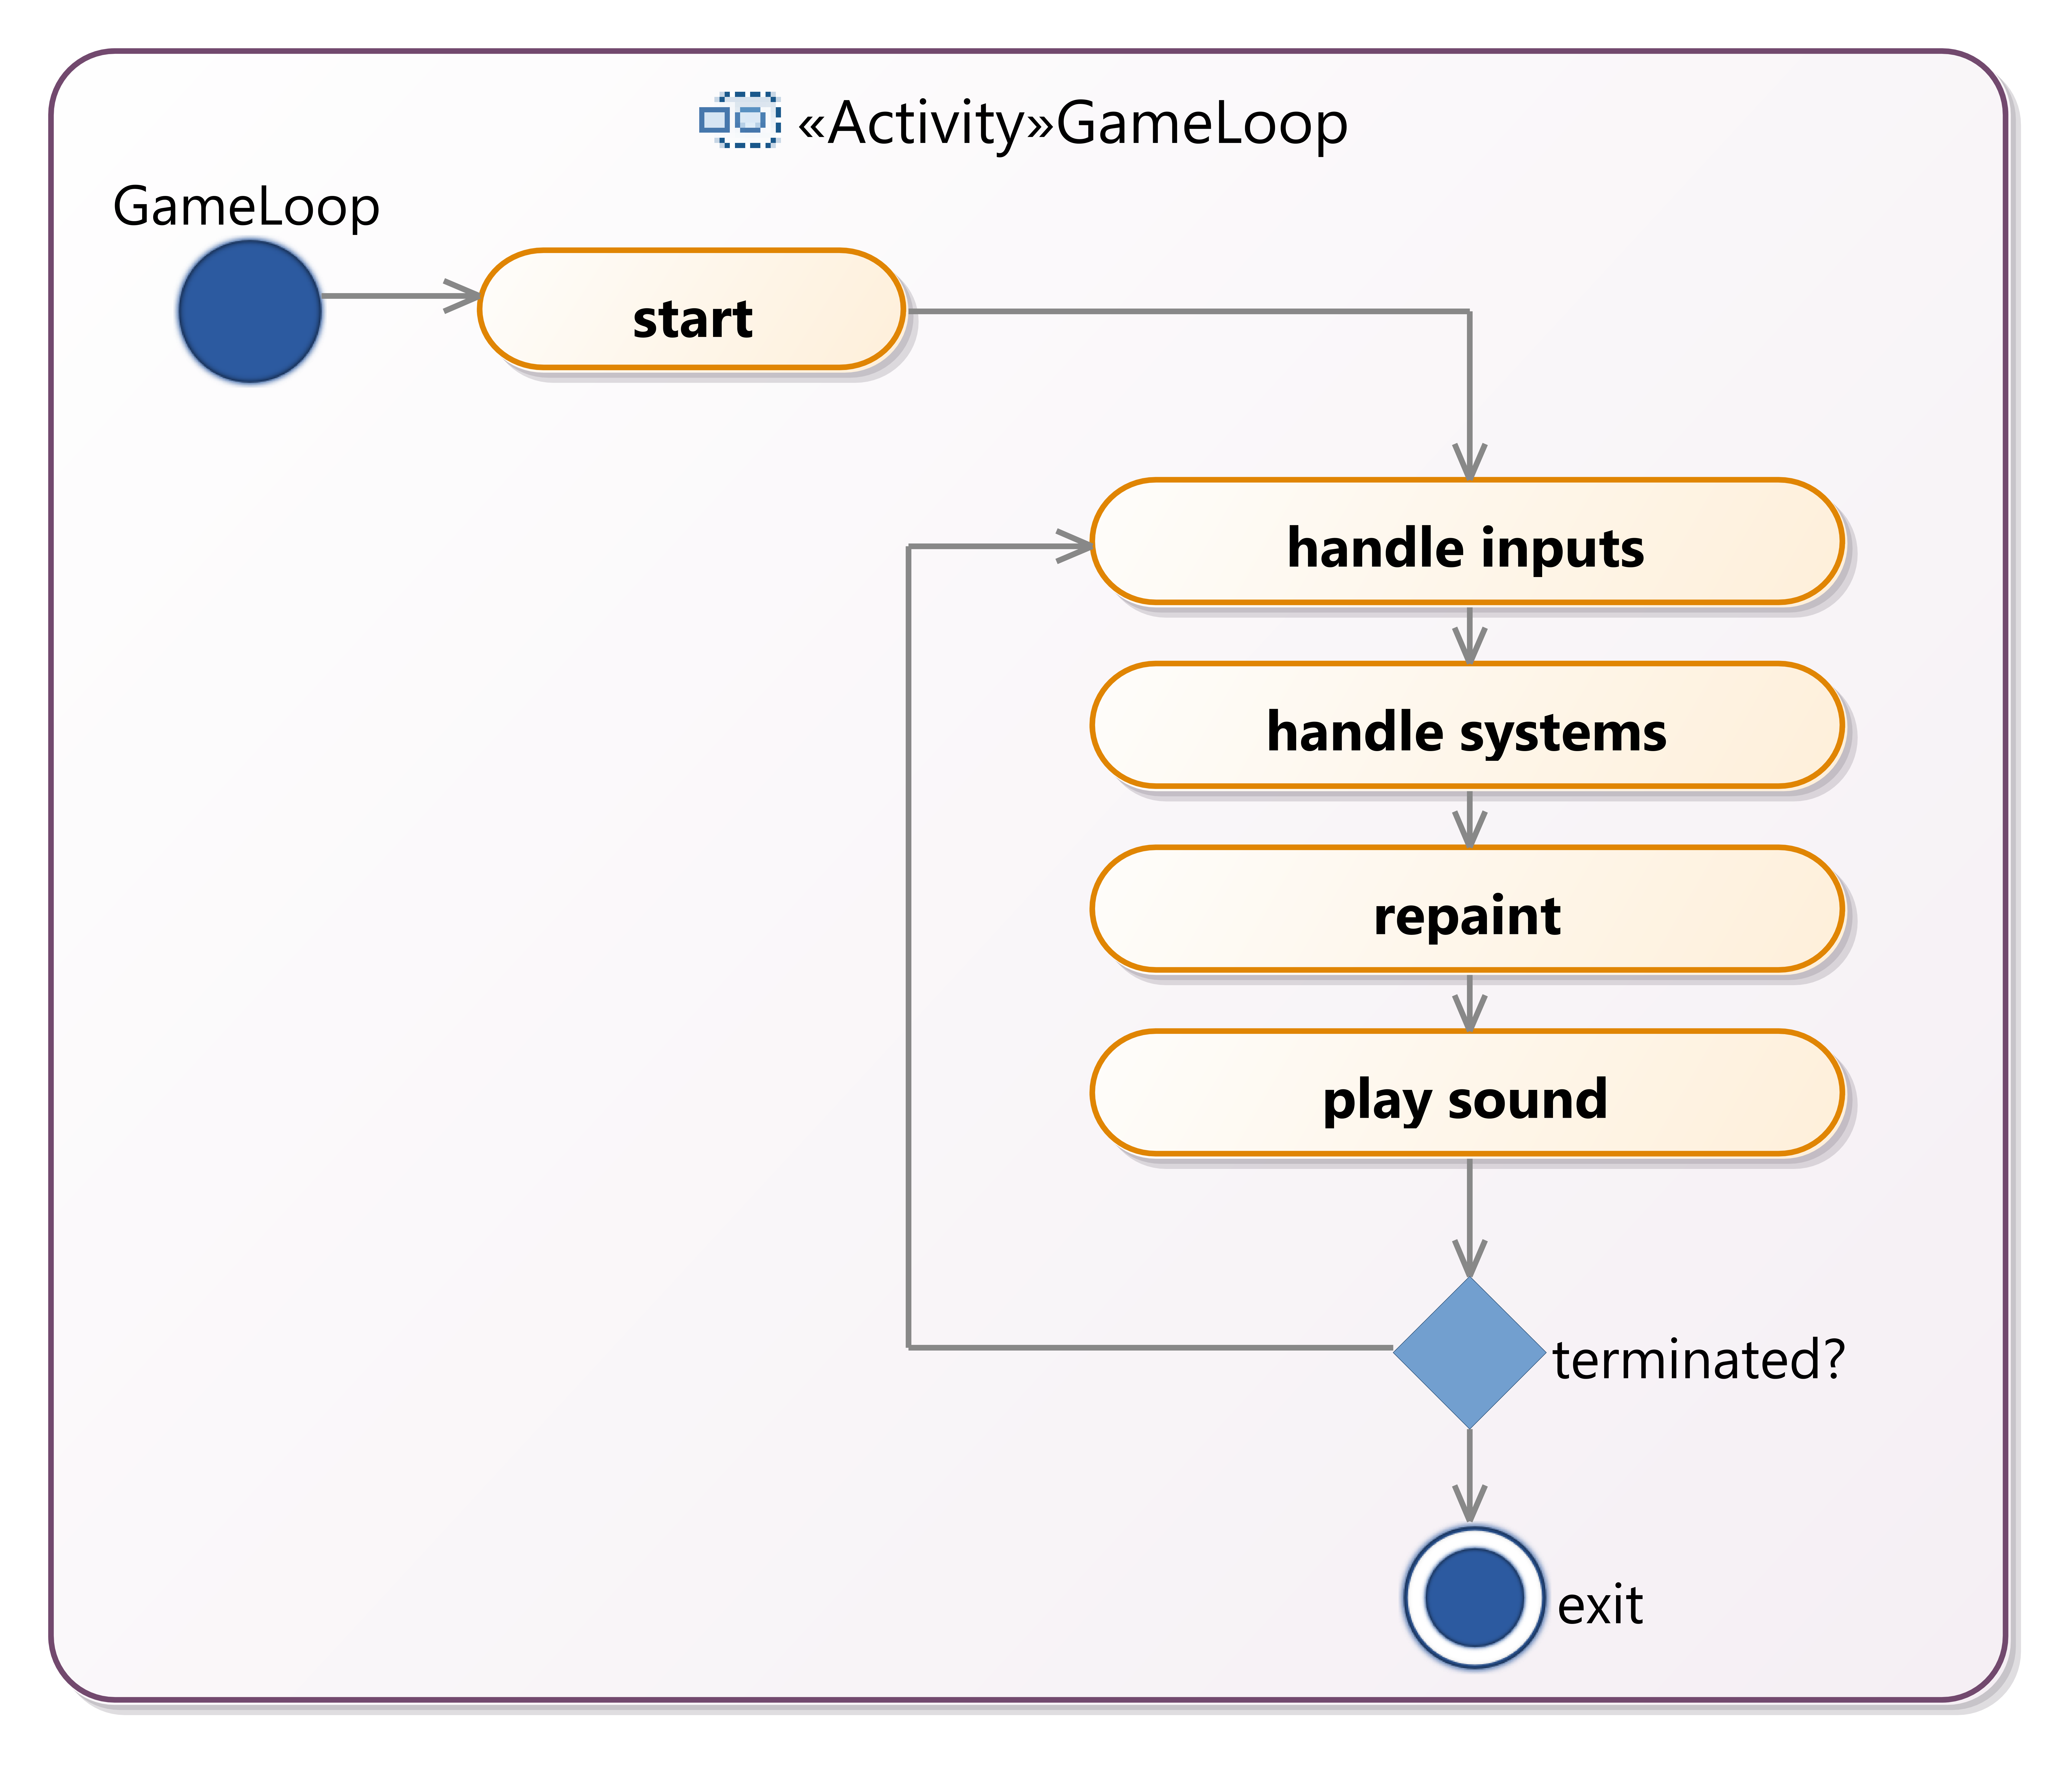
\includegraphics[width=\textwidth]{Pictures/res/implementation/gameloop-process}
    \caption{Game loop execution order}
    \label{fig:gameloop-process}
\end{figure}

\subsection{Input Recording}\label{subsec:input-recording}
Input recording is executed in a separate thread and handles inputs at a rate of $\Delta t_{inputs} = 20 ms$, since inputs in between two frames
would otherwise not be received by the games' input handling system.
$20 ms$ is a delta time that was found to be working best with the given circumstances.
It records all user inputs correctly while preventing unused overhead from recording more events than usable by the game systems.
\\
Generally, a button press needs to be differentiated from a button click.
While a button press is a continuous event, a button click is a one time event defined as the state change from button is not pressed to button is pressed.
Each recorded event, either from \textit{ActionListeners} implemented directly on the \textit{RenderingPanel} or from
the \textit{GamePadAdapter} are queued to the engines \textit{InputManager} as explained in section~\ref{subsec:input-handling}.
\\
The game pad integration is explained in section~\ref{subsec:gamepad-integration}, as this section mainly focuses on the recording of inputs itself.
\subsection{Input Handling}\label{subsec:input-handling}
The \textit{InputManager} contains a list of all \textit{Handlers} available to the game, implements methods to add and remove objects
of the \textit{Handler} class and methods to queue events
to a list of events per type - \textit{MouseEvent}, \textit{KeyEvent} and \textit{InputAction} (controller inputs).
\\
Each \textit{Handler} connected to the \textit{InputManager} receives all the events available in the respective event
queues at the given time step and execute their handling methods, which
then execute the actual actions on the game and its entities.
The handler class is an abstract class that can be extended to implement a variety of handlers, depending on the game requirements.
One specific handler class, the \textit{CollisionDetectionHandler} is implemented by default and allows for an easy implementation of hovering and clicking entities with a ColliderComponent.
It compares the current mouse position (given in the latest mouse event) and handles a potential collision with an Entity.

\subsection{System Handling}\label{subsec:system-handling}
\textit{Systems} are time-based and triggered with every update loop of the game.
\textit{Systems} do not have specific handling methods for input types, they operate solely time-based and execute a pre-defined logic.
They contain methods for different calculations, game logic or time-based events and actions.
Similar to the \textit{Handler} class, the \textit{System} class is an abstract class that can be extended from to implemented system classes according to the game requirements.
The \textit{ActionSystem} is already implemented, which is used to handle different types of actions that can be triggered e.g.\ by pressing a button entity, which starts
another scene.
The reason for this system being time based instead of event based is, that the \textit{CollisionDetectionHandler} already sets the state of the components,
however possible \textit{ActionComponents} need to be handled as well.
If a \textit{CollisionObject} is clicked or hovered, the \textit{ActionSystem} will check for possible actions to execute available from the \textit{ActionComponent}.

\subsection{Scene Update \& Repaint}\label{subsec:scene-update-&-repaint}
The next step in the game loop is a generic update of the currently active scene, which may be removing any unnecessary entities based on different conditions or
checking for a state change after an input or action has been handled.
After the update, the active scene is repainted by the \textit{RenderingEngine}~\ref{subsec:graphics-engine}.

\subsection{Rendering Engine}\label{subsec:graphics-engine}
The \textit{RenderingEngine} is a static class implemented within the game engine to handle all visible objects, screen rendering and scaling.
All content is rendered to a \textit{JPanel} object by using the \textit{Graphics2D} instance available by default, this is called the \textit{RenderingPanel}~\cite{jpanel,graphics2d}.
\\
The \textit{RenderingEngine} receives scaling factors for width and length from the \textit{ScalingEngine} and the \textit{RenderConfiguration}
classes, which handle resizing the frame,
fullscreen mode and different screen resolutions as well as antialiasing options.
During the rendering cycle, every location and boundary of the \textit{RenderObjects} is scaled and only afterwards it is rendered, however the original design position
is always present in the \textit{RenderObject} parameters.
This is necessary to correctly handle rescaling.
\\
A rendering cycle executes a few different methods which are all called by the overwritten repaint method from the \textit{RenderingPanel}.
First, all entities with a \textit{RenderComponent} are queried by the \textit{Query} system of the game engine and added to the rendering stack.
This stack is then split up into multiple stacks of \textit{RenderObjects}, which are the objects saved to the component that describe the actual
graphical visualization, based
on their rendering layer.
Each layer is rendered one after another by using specific rendering classes for different objects such as images, text or shapes.
Layering allows for stacking of multiple graphical entities above each other and allows for a better design and development flow GUIs and the game itself,
as the order of implementation and creation of entities is made obsolete through the usage of layers.
The following layers are rendered in this order:
\begin{enumerate}
    \item Background
    \item Game Layer 1
    \item Game Layer 2
    \item Game Layer 3
    \item Game Hover Layer
    \item UI Layer 1
    \item UI Layer 2
    \item UI Hover Layer
\end{enumerate}
For example, if a simple composition of background image, game entity and UI should be rendered at the same position,
the UI will always be in front of the game entity located at any of the game layers,
while the game entity will always overwrite the background at that position.
The reason for multiple UI and Game layers is simply to allow for a greater variety and range of possibilities when it comes to designing the game scenes.
\todo{add figure}.
\subsection{Sound Engine}\label{subsec:sound-engine}
A \textit{SoundEngine} is implemented in the game engine, which handles playing, pausing and stopping any audio stream available.
During each cycle, the \textit{SoundEngine} collects all entities with a \textit{SoundComponent} available, and checks if they are already playing and if not, if they should be playing.
The \textit{Java} built-in library \textit{Clip} is used to play audio streams and loop them if necessary~\cite{clip}.
This allows for an easy handling of any sound that should be played during a game, e.g.\ background music or button click sounds.

\subsection{Utility Classes}\label{subsec:utility-classes}
Detached from the \textit{GameLoop} execution, there are also multiple other configuration classes, managers, systems and utility classes, which will be briefly explained in this chapter.
\subsubsection{Game Configuration}\label{subsubsec:game-configuration}
The \textit{GameConfiguration} class by default implements a random profile name chosen of a variety of different names at game start, which is then used for saving high-scores
or may also be used in other parts of the game.
It also contains parameters for the currently active language, rendering configuration and sound configuration.

\subsubsection{Game Information}\label{subsubsec:game-information}
In the \textit{GameInformation} class, some generic variables for a title of the game, authors, version and description can be set, which are then used for instance as the games frame
title.

\subsubsection{Scene Manager}\label{subsubsec:scene-manager}
The \textit{SceneManager} is the main storage of all scenes, which may be menu scenes such as main menus or level scenes, i.e.\ game maps.
It can be called from anywhere within the game to switch a scene to another loaded scene or add a new scene to the scene stack.
Scenes should have unique identifiers (ids) in order for the \textit{SceneManager} to correctly load scenes from the stack.
\subsubsection{Resource Manager}\label{subsubsec:resource-manager}
The \textit{ResourceManager} is used for loading any kind of resource from outside the \textit{Java} classes, e.g.\ audio files, images or xml data and processes
these resources accordingly.
There are multiple implementations which are used by the \textit{ResourceManager} for loading of different XML files,
such as high-scores (\textit{HighScoreManager}) or languages (\textit{LanguageManager}),
however the basic implementation of the \textit{ResourceManager} equals their implementation and therefore the XML
parsing and processing is going to be described only for the \textit{ResourceManager}.
The following resource can be loaded by the resource manager and its sub manager classes:
\begin{itemize}
    \item Images, using the method \textit{loadImage()}
    \item Fonts, using the method \textit{loadFont()}
    \item Maps, using the method \textit{loadLevel()}
    \item Tilesets, using the method \textit{loadTileset()}
    \item Scores, using the method \textit{loadScores()}
\end{itemize}
\subsubsection{Logging}\label{subsubsec:logging}
The \textit{Java} logging tool is available and easily accessible from any class by simply using the static function
implemented in the \textit{Game} class and adding information to
the logger, which needs a specified log level and message to log.
Logging is and should always be implemented in stages of the game such as start, close or critical calculations, to identify possible bugs
easier.
\subsubsection{Styling \& Design}\label{subsubsec:styling-&-design}
A basic color scheme and font collection is already directly implemented to the game engine and may be used from scratch,
without loading other fonts or having to think about
color schemes.
This allows for a quick and easy design of graphical components.
\section{Game Implementation}\label{sec:game-implementation}
This chapter delves into the actual implementation of the game, highlighting the instances where the generic game engine is
employed and the reasons behind its use.
Additionally, it provides a comprehensive explanation of the various systems implemented to compute the game mechanics.
\subsection{Handler}\label{subsec:handler}
\textit{Handlers}, as already pointed out, are used to handle user inputs and trigger certain things within the game.
The implemented handlers for the game will be explained in this chapter.
\subsubsection{Build Handler}\label{subsubsec:build-handler}
The \textit{BuildHandler} is used to handle the placement, replacement, removal and connection of components to the game grid.
There are different \textit{SimulationTypes}, which are handled differently.
For the component and cable placement, the following constraints apply:
On each game grid tile, there may only be exactly one component of type \textit{ACTUATOR}, \textit{SENSOR}, \textit{COMPUTER} or \textit{VOTER}.
If any of the above-mentioned components exists on a tile, no cable may be placed at this position.
CABLE type components are handled differently, as there may be cables of different types (red, blue, green, yellow) on the same tile, to enable
cross strapping of different components.
Cables can be rotated at both ends to correctly connect components as wanted.
Whenever a cable or component is placed or rotated, the connections are updated.
To display this connection, cable ports are used.
Each cable port can be used to connect a single other entity to the cable port.
Sensors have 4 cable ports with the type output, respectively actuators have 4 cable ports with type input.
Computers and voters have in and out puts, whereas cables only have a single in and output.
When replacing or removing a component, the removed component will be put back to the build panel and may be used again.
\todo{flow besser beschreiben}
\subsubsection{CursorSelectorHandler}\label{subsubsec:cursorselectorhandler}
For handling game pad and keyboard inputs, the \textit{CursorSelectorHandler} was implemented.
It creates a globally available entity (meaning, it is available in every scene), which displays a virtual cursor that can be
moved around by using the keyboard arrows or the joysticks of a gamepad.
It handles all input actions coming from gamepads and key events coming from the keyboard, and converts them to their according mouse events,
if necessary and defined.
This way, all other handler implementations only need to handle mouse events, which are virtually queued from the cursor selector handler.

\subsection{System}\label{subsec:system}
\subsubsection{Simulation System}\label{subsubsec:simulation-system}
The \textit{SimulationSystem} handles updates of the current components on the game field, as well as starting the game goal
validation by using the \textit{MarkovProcessor}, as explained in section~\ref{subsubsec:example-markov-chains}.
\\
Each cycle of the \textit{SimulationSystem} executes four different methods.
At first, the group ids of each simulation entity are updated, as well their input ids.
This is needed in order for every entity to know to which other entities they are connected, which is necessary to correctly
update their states, both during the building mode and during the Markov simulation, where these connections are copied.
After updating the state, the graphical representation of each state is changed, depending on the actual state.
This shows, if an entity is correctly connected and working, or if it is currently not connected.
\\
The Markov chain computation is executed in a separate thread, which enables accurate rendering of animations during
the calculation, such as the aircraft's movement through the sky.
Once the Markov chain calculation is complete, all states that result in a system failure - taking into account the level goal and
requirements (minimum functional components, system failure probability, maximum out-of-control components) - are identified and
summed up to determine the system failure probability.
This probability is calculated separately for both out-of-control and passive failures.
\\
Subsequently, if the probabilities align with the level target and the validation is successful, the total score is calculated using the probabilities,
the remaining components in the build panel, and a base level score.
\\
Each level has a predetermined base score upon completion.
\begin{equation}
    s_{base} = 100
    \label{eq:base-score}
\end{equation}
The probabilities of the current state calculated are compared to the target requirement failure probability by comparing the number of exponentials of 10 to each other.
\begin{equation}
    s_{accuracy} = 10 \cdot \lvert \log_{10} p(state) - \log_{10} p(goal)\rvert
    \label{eq:accuracy-score}
\end{equation}
The component score is defined as the sum of all components that are still available to the player in the build panel (excluding cables).
\begin{equation}
    s_{component} = \sum_{i = 1}^{n_{components}} 10
    \label{eq:component-score}
\end{equation}
The total score is the sum of the three previously calculated scores.
\begin{equation}
    s_{total} = s_{base} + s_{accuracy} + s_{components}
    \label{eq:total-score}
\end{equation}
Each score is shown separately in the score overview, with an additional indication of the accuracy of the probabilities to the target.
The user can see, where he or she may improve the system in order to get closer to the target.
This scale is also shown, when the validation of the target requirements is not passed by the currently built system, to indicate
a hint on what could be improved by the user.
\\
To correctly validate the goal, the actual probability calculated is summed up with an epsilon value of $\epsilon = 1e-7$,
to prevent incorrect validations due to rounding errors in double values.
The double precision floating point error occurs due to the internal representation, which can only represent a specified range of
values~\cite{floating-point}.
Therefore, especially when working with very small or very large numbers, rounding errors (i.e.\ the next representable value by the internal structure which can be stored
in the binary format) occur.
\subsubsection{Markov Processor}\label{subsubsec:example-markov-chains}
In this chapter, some examples for Markov chains that represent the level designs will be shown and the implementation of the
\textit{MarkovProcessor} will be explained by using these graphs.
\\ \\
The \textit{MarkovProcessor} generates a markov chain, based on the given entities and available groups and inputs provided by the \textit{SimulationSystem}.
First, a starting state, including all the relevant \textit{Entities} is generated.
Each state is represented as a \textit{MarkovState}, which contains the probability of the state occurrence, equalling the
transition rate, and a list of \textit{MarkovStateObjects},
that represent the different entities available after validating
the current level.
This step is needed in order to generate all the different \textit{MarkovStates} without actually modifying the game grid.
\\ \\
For demonstration purpose, a simple system state with a single sensor, computer and actuator is used.
Whenever a failure state is update to \textit{passive} or \textit{out-of-control}, all other components will also be updated accordingly,
which can also be seen in figure~\ref{fig:markov-simplex}.
The indices used are as follows: S = Sensor, C = Computer, A = Actuator.
The failure probabilities of each component is:
\begin{equation}
    \lambda_{f,S} = 1\text{e-}4
    \label{eq:markov-1}
\end{equation}
\begin{equation}
    \lambda_{f,C} = 1\text{e-}4
    \label{eq:markov-2}
\end{equation}
\begin{equation}
    \lambda_{f,A} = 0
    \label{eq:markov-3}
\end{equation}
For the failure detection ratio, the following values are used:
\begin{equation}
    C_{S} = 0.9
    \label{eq:markov-4}
\end{equation}
\begin{equation}
    C_{C} = 0.9
    \label{eq:markov-5}
\end{equation}
\begin{equation}
    C_{A} = 1
    \label{eq:markov-6}
\end{equation}

\begin{figure}
    \begin{center}
        \scalebox{0.33}{
            \begin{tikzpicture}[->, >=stealth', semithick, node distance=7cm, auto]
            \tikzset{rectangle/.append style={draw=black, thick, fill=white}}
            \node    (S)[font=\fontsize{24}{0}\selectfont]  {\TBox[fill=white]{Sensor}};
            \node    (C)[font=\fontsize{24}{0}\selectfont, right of=S]  {\TBox[fill=white]{Computer}};
            \node    (A)[font=\fontsize{24}{0}\selectfont, right of=C]  {\TBox[fill=white]{Actuator}};
            \path
    (S) edge (C)
    (C) edge (A)
            \end{tikzpicture}
        }
    \end{center}\caption{Example System System}
    \label{fig:simplex}
\end{figure}


\begin{figure}
\begin{center}
    \scalebox{0.33}{
        \begin{tikzpicture}[->, >=stealth', semithick, node distance=7cm, auto]
        \tikzset{rectangle/.append style={draw=black, thick, fill=white}}
        \node    (A)[font=\fontsize{20}{0}\selectfont]  {\TBox[fill=white]{C}\TBox[fill=white]{C}\TBox[fill=white]{C}};
        \node    (B)[font=\fontsize{20}{0}\selectfont,below of=A]   {\TBox[fill=white]{C}\TBox[fill=white]{F}\TBox[fill=white]{C}};
        \node       (C)[font=\fontsize{20}{0}\selectfont,left of=B] {\TBox[fill=white]{F}\TBox[fill=white]{C}\TBox[fill=white]{C}};
        \node (D)[font=\fontsize{20}{0}\selectfont,right of=B] {\TBox[fill=white]{C}\TBox[fill=white]{C}\TBox[fill=white]{F}};
        \node (G)[font=\fontsize{20}{0}\selectfont,below left of=B] {\TBox[fill=white]{C}\TBox[fill=blue!30]{P}\TBox[fill=blue!30]{P}};
        \node (H)[font=\fontsize{20}{0}\selectfont,below right of=B] {\TBox[fill=white]{C}\TBox[fill=red!30]{O}\TBox[fill=red!30]{O}};
        \node (F)[font=\fontsize{20}{0}\selectfont,left of=G] {\TBox[fill=red!30]{O}\TBox[fill=red!30]{O}\TBox[fill=red!30]{O}};
        \node (E)[font=\fontsize{20}{0}\selectfont,left of=F] {\TBox[fill=blue!30]{P}\TBox[fill=blue!30]{P}\TBox[fill=blue!30]{P}};
        \node (I)[font=\fontsize{20}{0}\selectfont,right of=H] {\TBox[fill=white]{C}\TBox[fill=white]{C}\TBox[fill=blue!30]{P}};
        \node (J)[font=\fontsize{20}{0}\selectfont,right of=I] {\TBox[fill=white]{C}\TBox[fill=white]{C}\TBox[fill=red!30]{P}};
        \path
    (A) edge[font=\fontsize{20}{0}\selectfont,left,pos=0.8]     node{$\dot{p_2}=\lambda_{f,C} \cdot p_1$}     (B)
        edge[font=\fontsize{20}{0}\selectfont,above left,pos=0.2]    node{$\dot{p_3}=\lambda_{f,S} \cdot p_1$}      (C)
        edge[font=\fontsize{20}{0}\selectfont,above right,pos=0.2]    node{$\dot{p_4}=\lambda_{f,A} \cdot p_1$}      (D)
        (C) edge[font=\fontsize{20}{0}\selectfont,above left,pos=0.5] node{$p_5=\dot{p_3} \cdot C_S$} (E)
        edge[font=\fontsize{20}{0}\selectfont,below right,pos=0.6] node{$p_6=\dot{p_3} \cdot (1-C_S)$} (F)
        (B) edge[font=\fontsize{20}{0}\selectfont,above left,pos=0.4] node{$p_7=\dot{p_2} \cdot C_C$} (G)
        edge[font=\fontsize{20}{0}\selectfont,above right,pos=0.4] node{$p_8=\dot{p_2} \cdot (1-C_C)$} (H)
        (D) edge[font=\fontsize{20}{0}\selectfont,below left,pos=0.8] node{$p_9=\dot{p_4} \cdot C_A$} (I)
        edge[font=\fontsize{20}{0}\selectfont,above right,pos=0.5] node{$p_{10}=\dot{p_4} \cdot (1-C_A)$} (J)
        \end{tikzpicture}
    }
\end{center}
\caption{Markov Chain Simplex System}
\label{fig:markov-simplex}

\end{figure}
The markov chain for these parameters can be seen in figure~\ref{fig:markov-simplex}.
\\
The implementation starts by generating a starting node, where all states are set to correct for the available components.
This state has a set probability of 1.
For each new state, the transition probability to this state from the previous state is calculated by multiplying the previous state probability with the
failure probability of the current failed component.
From there, each branch splits into two branches, one taking into consideration the failure detection ratio to calculate the passive failure state,
the other for calculating the out-of-control failure state.
\\
The approach of the implementation always sets the previous and the next states from a current state accordingly, so the tree-like
graph can be searched for specific states and state transitions.
Eventually, to receive the failure probability for a given state or a given set of states (e.g.\ all states that lead to a system failure), there is an algorithm
that finds exactly these states and calculates the sum of their probabilities.
Here, the failure probability for a time step of $t = 1 \text{h}$ is used, which results in a simplification of the general equations that removes all the integrations.
Therefore, only the state transition probabilities have to be summed up to calculate the actual probability for a specific set of states that can or cannot occur.
For larger or smaller time steps, instead of directly adding up the state transition probabilities, one would need to integrate the probability n times, based on the amount of nodes
/ states that are previous to each state.
\\
\\
A challenge during the implementation was the performance optimization for markov chains with increasing amount of system components.
There are two different approaches to the implementation, which are described below.
Additionally, an additional technique called ``Memoization'' is used to increase the performance even further.
\textbf{Recursive Markov Chain Generation}\\
New \textit{MarkovStates} are generated recursively, by calling the method from within the method directly after creating
and adding a new state to the next state list of a \textit{Markov State}.
This is calculated, until the break criteria is reached, which is, when a branch of the train is calculated until its very end,
where all \textit{MarkovStateObjects} are in
one of the two failed states, either OUT-OF-CONTROL or PASSIVE\@.
\textbf{Iterative Markov Chain Generation}\\
In the same way that states are calculated recursively, the same method was also implemented in an iterative manner,
after performance issues occurred with the recursion.
This is implemented via a stack, which is iterated through until it is empty.
With each iteration, new \textit{MarkovStates} are added to the stack, until each branch is finished, i.e.\ all \textit{MarkovStateObjects}
are in a failed state.
\textbf{Memoization}\\
To further optimize the algorithm, memoization was implemented.
Memoization is a programming technique used to optimize the execution time of computationally expensive functions by caching
their results for a given set of input parameters~\cite{10.5555/971738.971743}.
When a memoized function is called with the same input parameters as a previous call, the cached result is returned instead of re-computing the function.
In the implementation, a \textit{HashMap} is used, that stores each \textit{MarkovState} as a key-value pair by using a hash code
calculated from the current \textit{MarkovStateObjects} states.
Whenever another state change would require the \textit{MarkovProcessor} to calculate a state already available in this map, the \textit{MarkovState}
is instead cloned from there instead,
as the same \textit{MarkovState} means, that the exact same components have failed.

\subsection{Scene}\label{subsec:scenes}
A hierarchical scene structure was implemented to the game, which can be seen in figure~\ref{fig:scenes-hierachry}.
The base scene contains elements of the game that are visible in every scene, and therefore can be inherited to all other scene classes.
This includes the games background image and generic option buttons for settings, sound, back to menu and exit.
From this base scene, a base menu scene and a base game scene are inherited, which are used to display different menu screens and contain
the basic elements necessary to play the game or build maps in the build mode.
These scenes inherit multiple other scenes, which show different menus (main menu, level map, settings menu) and game scenes (main game scene, build mode scene, tutorial scene).
Specifically for tutorials, an interface which implements methods to display tutorial dialogues has been added to the game, which describes classes as tutorial classes.
Whenever a tutorial dialogue needs to be handled, this interface has to be implemented.

\begin{figure}
    \centering
    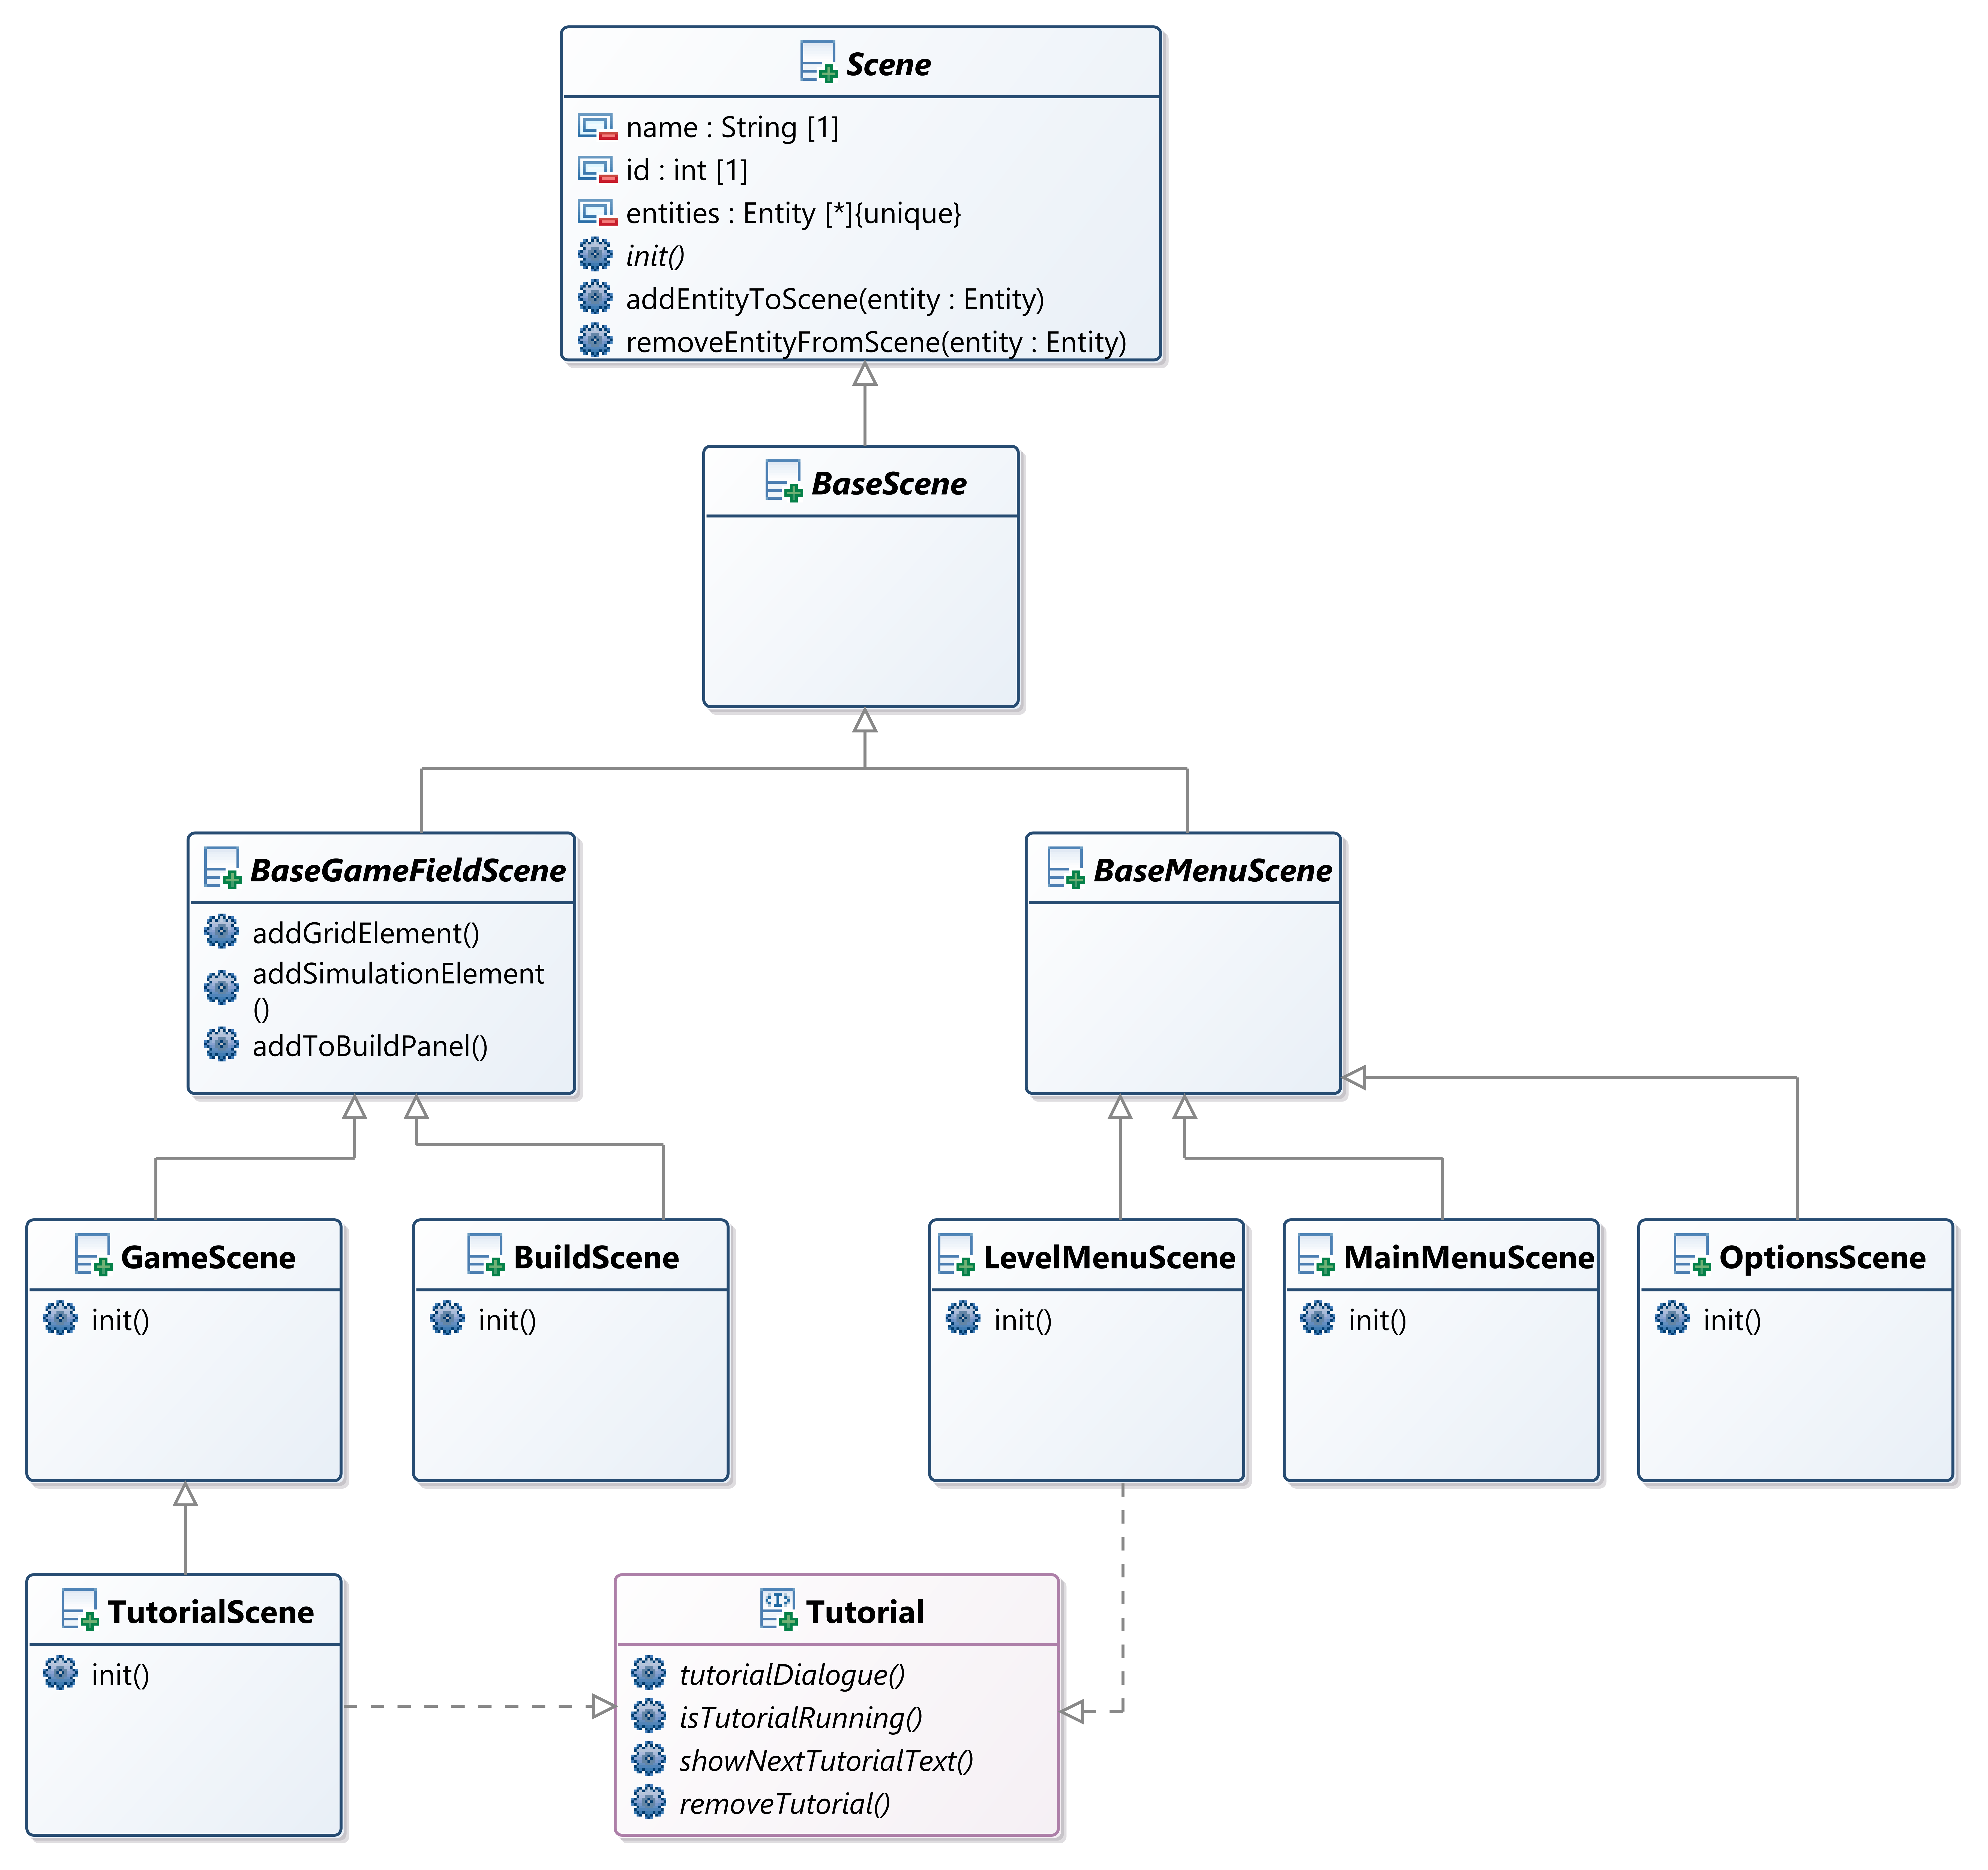
\includegraphics[width=\textwidth]{Pictures/res/implementation/scenes-hierarchy}
    \caption{Scene hierarchy}
    \label{fig:scenes-hierachry}
\end{figure}

The basic layout of the scenes was already described in~\ref{subsec:graphic-design}, the finished implementation of these
layouts is visualized in figures~\ref{fig:game-scene} and~\ref{fig:level-scene}.
Furthermore, the menu scene implementation is displayed in figure~\ref{fig:menu-scene}.
\\
During scene design, a bright color palette was chosen to make the game environment appealing and playful.
For some elements, the color scheme of the Institute of Aircraft Systems was used (aircraft background, logo design).
The font used for the textual parts of the game is \textit{joystix monospace}~\cite{joystix}, which is a ``[\ldots] pixel-style
typeface inspired by 1980s arcade video games.
It's a timeless style that began with Atari in 1976 and extended to a slew of manufacturers throughout the 1980s.
It became the de facto font choice anytime a designer wanted to express classic videogame iconography in the twenty-first century''~\cite{joystix}.
As the main goal was to design an 8-bit styled, retro-like game, the font choice here is relatively obvious to make.
\todo{figures wirklich so?}
\begin{figure}
    \centering
    \setlength{\fboxsep}{1pt}
    \setlength{\fboxrule}{1pt}
    \fbox{
        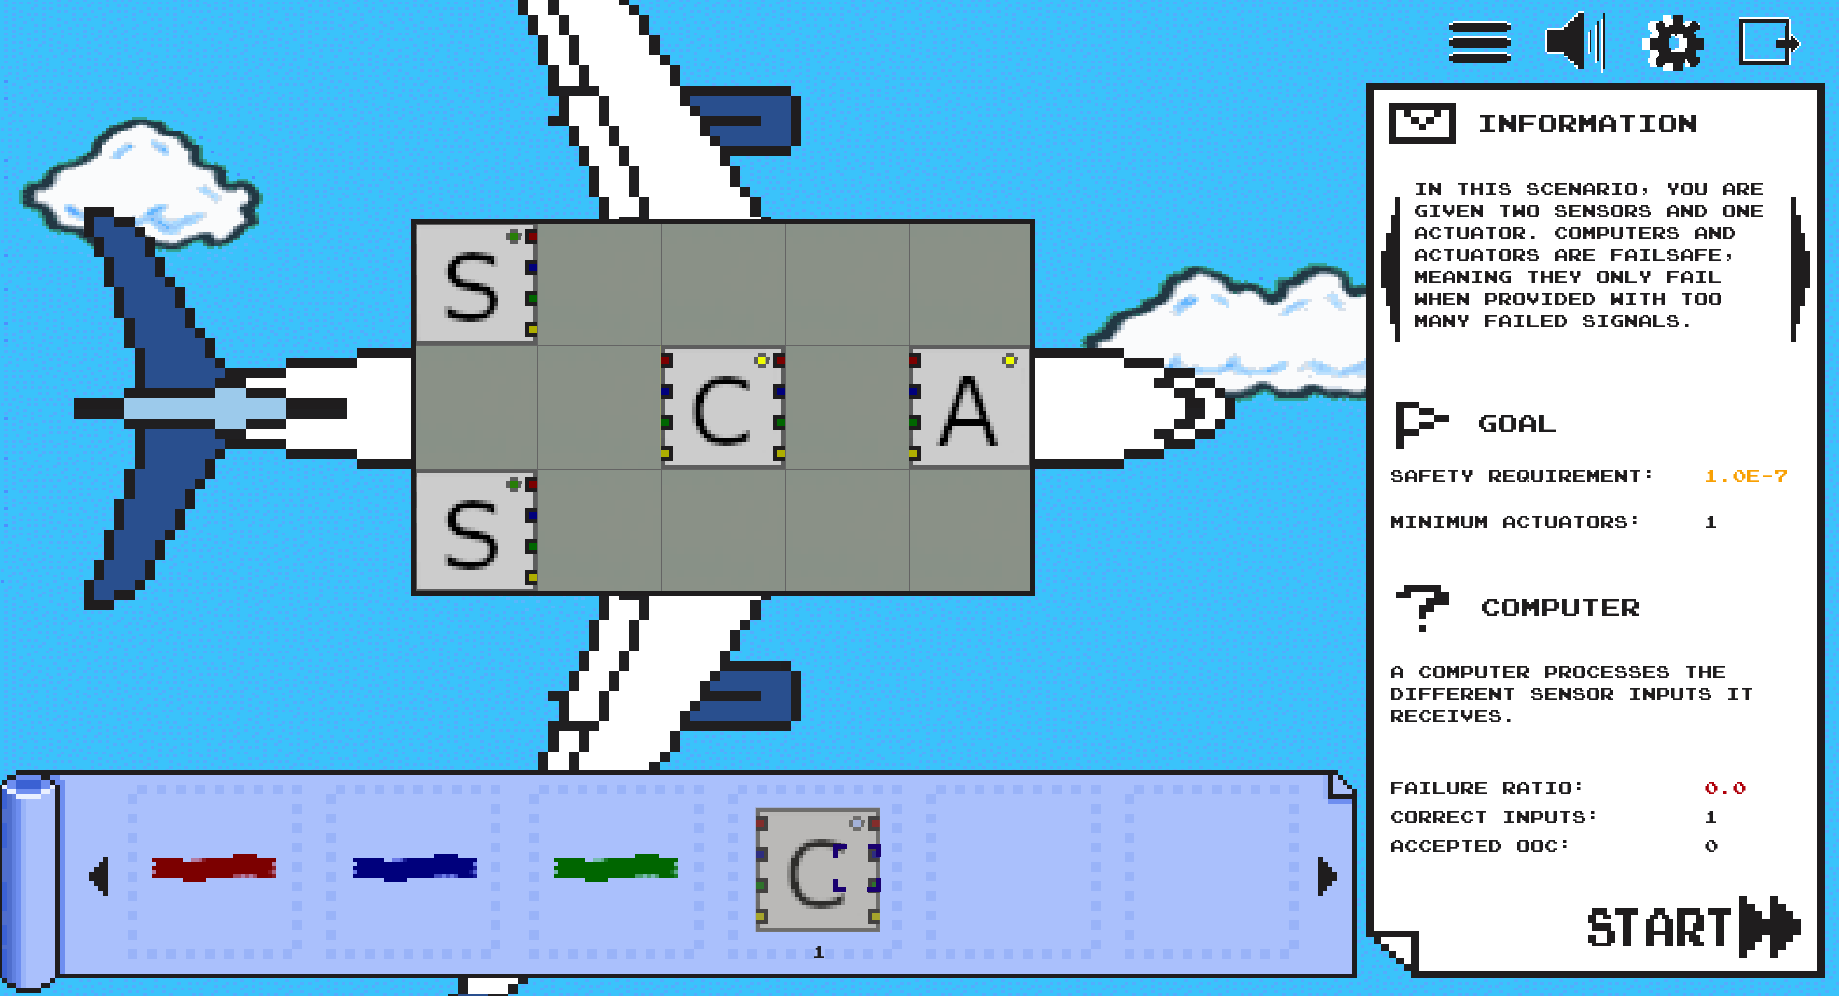
\includegraphics[width=0.9\textwidth]{Pictures/res/implementation/scenes/game-scene}
    }
    \caption{Game Scene}
    \label{fig:game-scene}
\end{figure}

\begin{figure}
    \centering
    \setlength{\fboxsep}{1pt}
    \setlength{\fboxrule}{1pt}
    \fbox{
        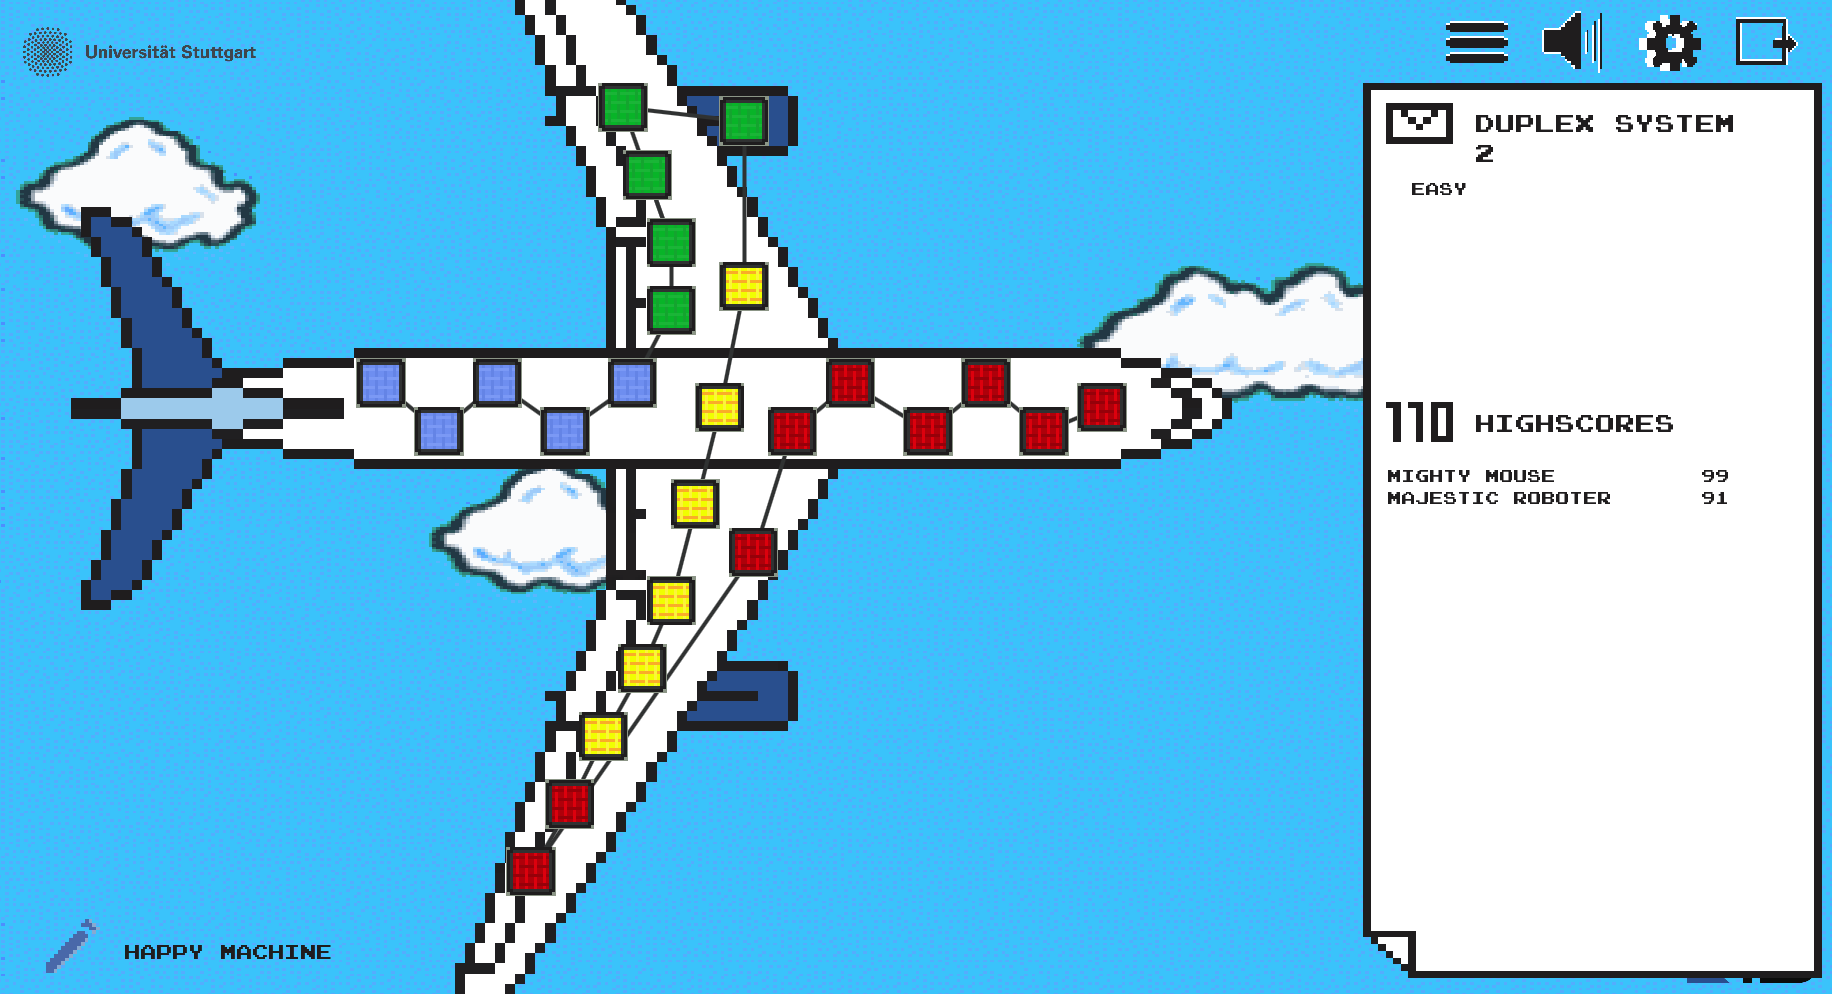
\includegraphics[width=0.9\textwidth]{Pictures/res/implementation/scenes/level-map}
    }
    \caption{Level Map Scene}
    \label{fig:level-scene}
\end{figure}

\begin{figure}
    \centering
    \setlength{\fboxsep}{1pt}
    \setlength{\fboxrule}{1pt}
    \fbox{
        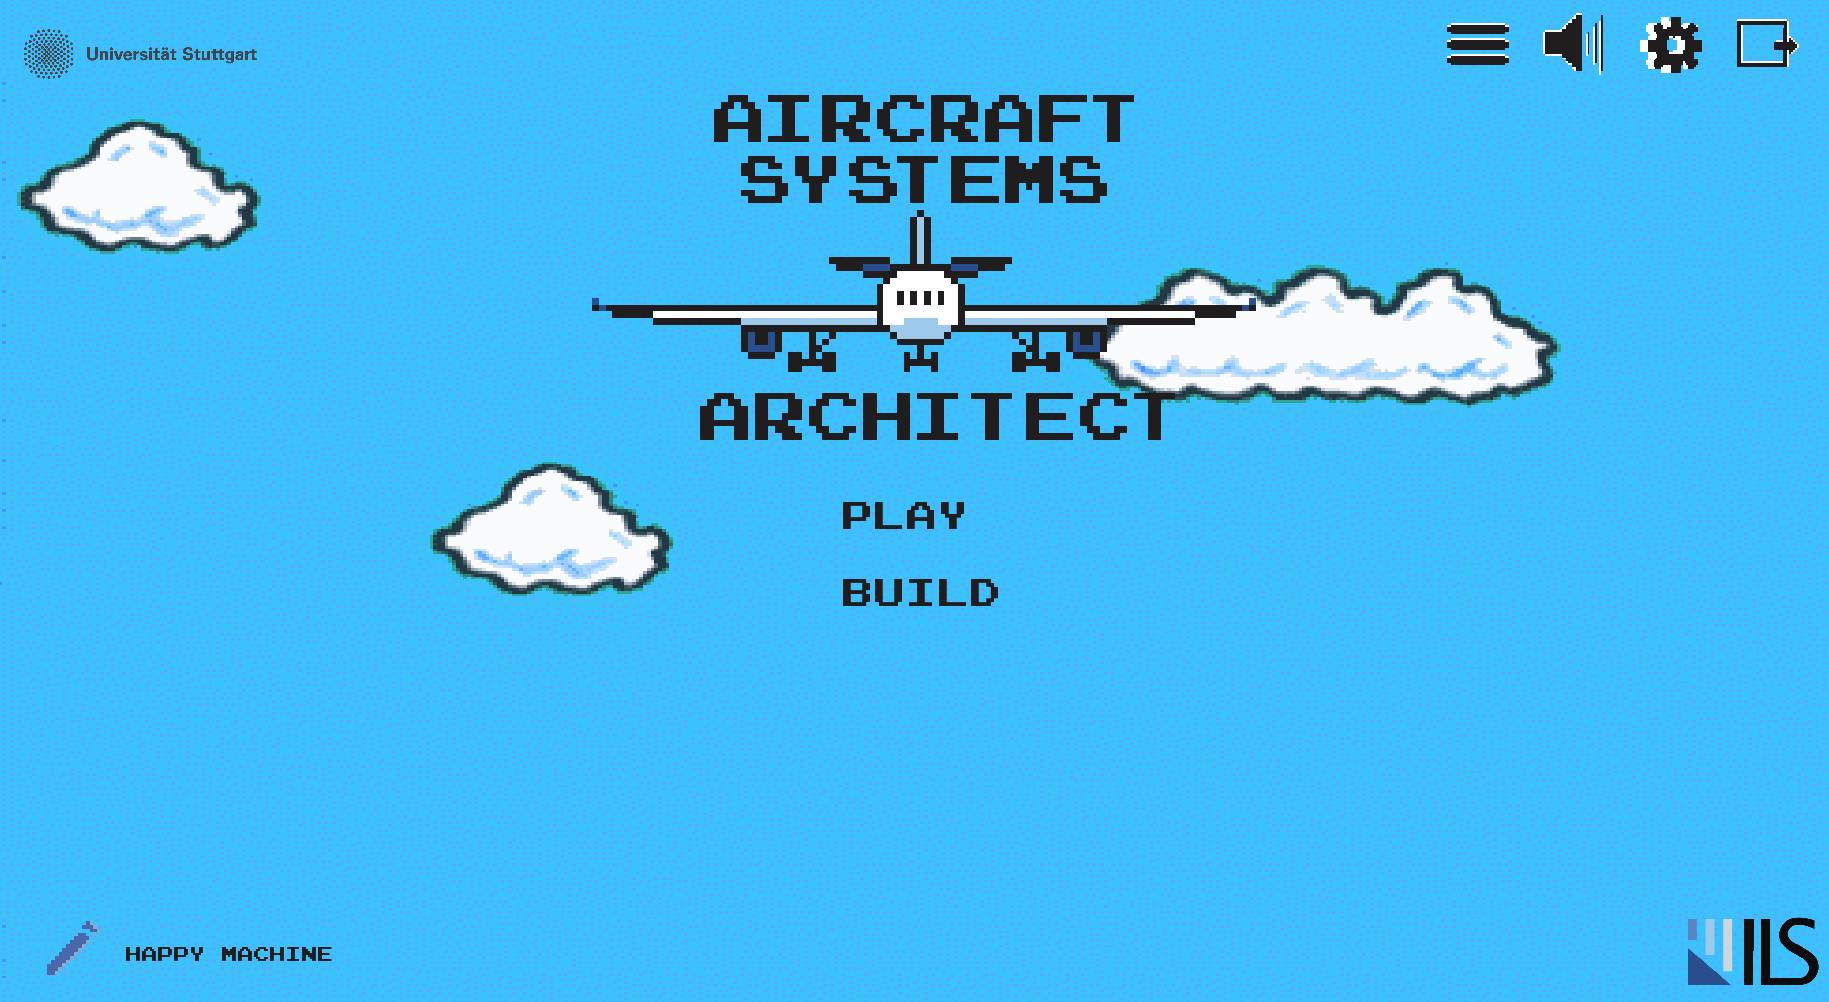
\includegraphics[width=0.9\textwidth]{Pictures/res/implementation/scenes/main-menu}
    }
    \caption{Menu Scene}
    \label{fig:menu-scene}
\end{figure}

\subsubsection{Entities}\label{subsubsec:entities2}
The entities in the games' scenes are implemented as generified objects that can be instantiated.
The following entities are currently available in the game implementation.
\textbf{Grid Entities:} \\
\textit{GridEntities} describe each tile of the grid, containing a grid position as $(x,y)$ coordinates and a customizable grid tile,
which is usually the regular concrete background, but may be changed any time for specific scenarios.

\textbf{Simulation Entities:} \\
All elements that are placed on the game grid are considered so-called \textit{SimulationEntities}.
These entities are built of components to describe the cable port distribution, parameters such as failure ratio and failure detection ratio and grid components, which contain the
entities position as a coordinate in the games' grid-like game field.
Each entity that should have a description on the right side tool box also has a \textit{TooltipComponent} attached, which indicates, that
a tooltip should be shown when hovering the entity.
Furthermore, graphics and colliders are available to simulation entity objects.

\textbf{Build Panel Entities:} \\
\textit{BuildPanelEntities} are entities which are available in the players' inventory and can be used for building objects on the game grid.
They include components for graphics description, build information - e.g.\ the failure ratio, failure detection ratio and amount in inventory,
and colliders.
Similar to the \textit{SimulationEntity}, a tooltip component is also available to the build panel entities to indicate tooltip descriptions.
\subsubsection{Components}\label{subsubsec:components2}
The above-mentioned entities implement different components to store the according data and to identify which component
should implement certain behaviors such as being able to be built to the grid or adding them to the simulation.
The following components were developed and implemented during the game development process.

\textbf{GridComponent:} \\
The \textit{GridComponent} stores the grid position as $(x,y)$ coordinates of an entity, where $x=0, y=0$ is the top left of the game grid.

\textbf{SimulationComponent:} \\
Data regarding the simulation run by the \textit{MarkovProcessor} is stored in the \textit{SimulationComponent}.
The simulation type (i.e.\ Actuator, Sensor, Computer, \ldots), as well as the current state (i.e.\ inoperative, correct by default, \ldots), failure
ratio and failure detection ratio are stored.
Furthermore, the component contains parameters to store the entity ids of entities connected as inputs to this component / entity, which is
not necessary, however enables easier maintainable code and performant look-ups for some systems.

\textbf{BuildComponent:} \\
The \textit{BuildComponent} is used to tell the systems operating the game, that an entity should be buildable.
Therefore, it contains similar information as the simulation component, as the parameters from the build component are used
to create new \textit{SimulationEntities} with \textit{SimulationComponents} attached when placing a component on the grid.
Furthermore, the \textit{BuildComponent} also stores the amount of components on the stack.
As this number would go below 0, no new component can be built.

\textbf{CablePortsComponent:} \\
\textit{CablePortsComponents} contain data regarding the connection of entities to each other.
Each \textit{CablePortComponent} can have multiple in- or outgoing cable ports.
\textit{CablePorts} are used to store another entity object, which describes the entity connect to another entity.
When updating a connection, both sides of the connection have to be considered.
A cable ports' connected entity parameter may be null, when there is currently no connection to the port.

\textbf{TooltipComponent:} \\
The \textit{TooltipComponent} may be used for entities that should display a tooltip upon hovering over the object with the cursor.
Information such as failure ratio, simulation type and description of the object are stored as text strings (as ids, which are read
from the language file, or as converted numbers to strings) in this component, so they may be directly used to render them to
the screen.
\subsubsection{Entity UML}\label{subsubsec:entity-uml}
A comprehensive overview of the different entity structures is given in figure~\ref{fig:entities}.
\begin{figure}
    \centering
    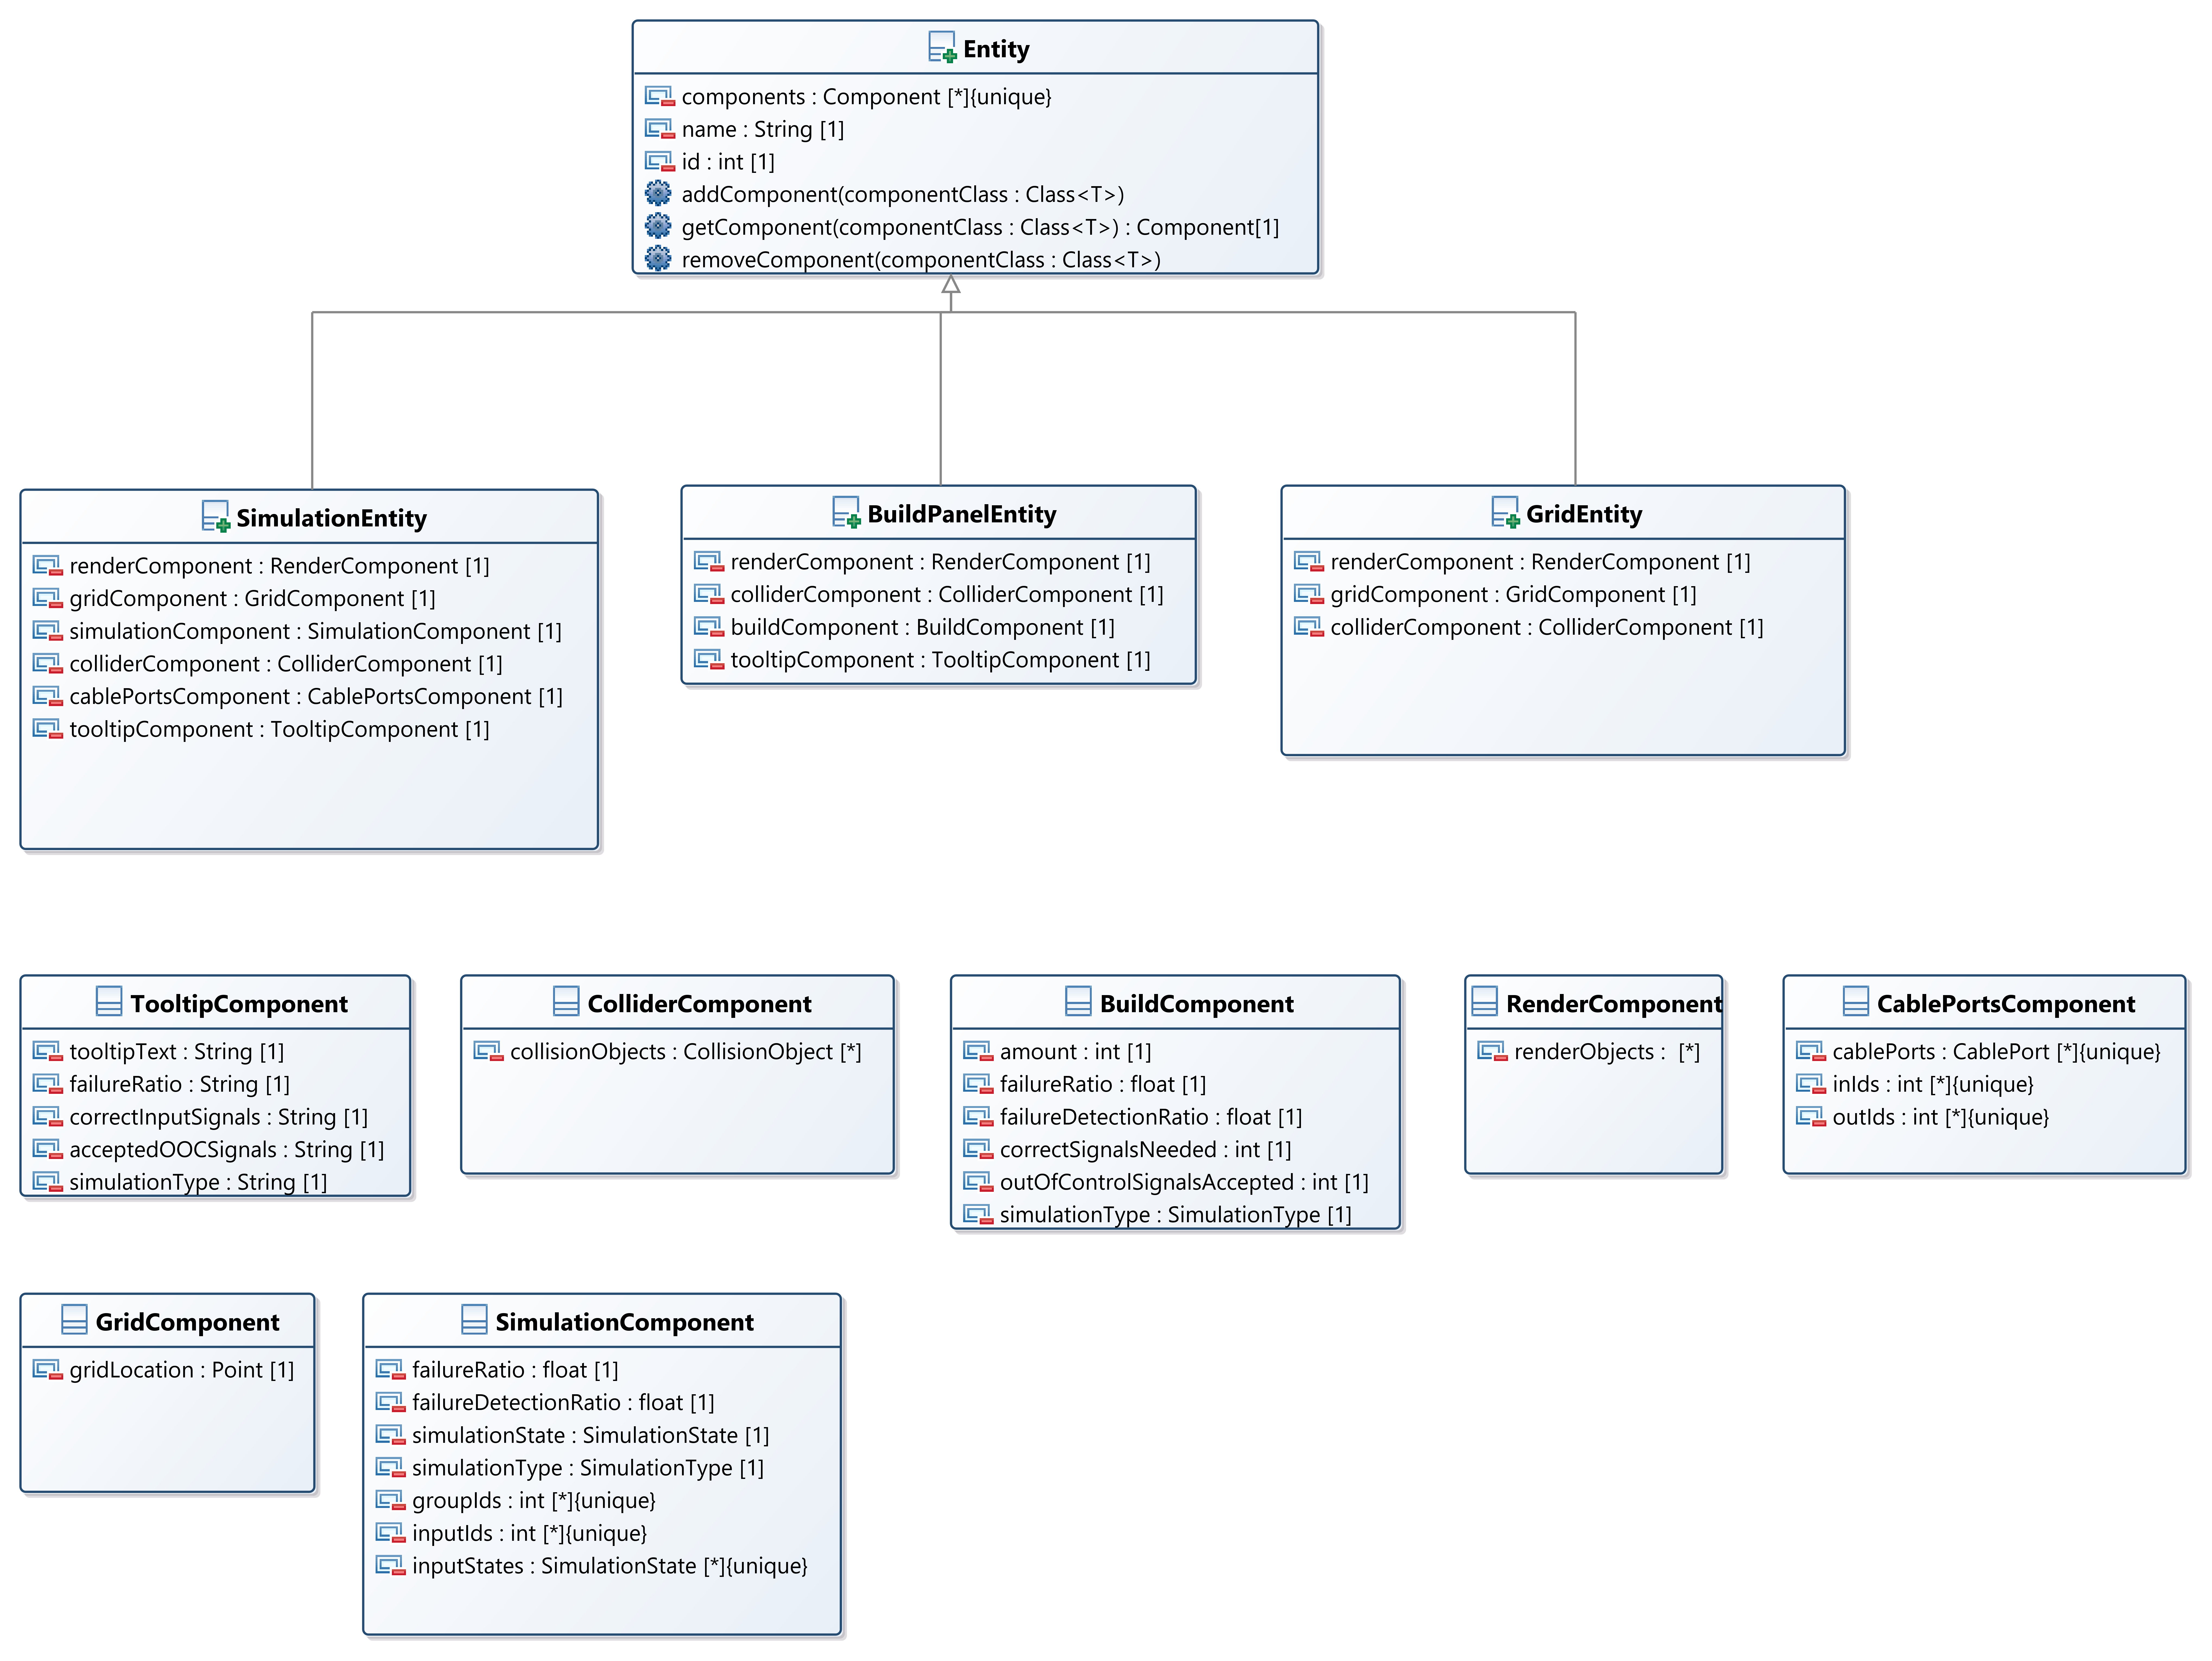
\includegraphics[width=\textwidth]{Pictures/res/implementation/entities}
    \caption{UML Diagrams of the different entities}
    \label{fig:entities}
\end{figure}
\subsection{Level Implementation}\label{subsec:level-implementation}
Each level is created as a new \textit{GameScene} object with the content of a level file that is read and parsed by the \textit{ResourceManager}
~\ref{sec:data-storage-&-data-parsing}.
The \textit{GameScene} object stores all relevant data, including the level requirements / goal, the grid size, available entities and,
if applicable through the
tutorial interface implementation, possible dialogues and character models that form the tutorial scene.
Following examples for different levels are provided in this chapter:
\begin{itemize}
    \item Tutorial Scene explaining the basics of the gameplay~\ref{fig:basic-gameplay-tutorial}
    \item Duplex System~\ref{fig:duplex-system}
    \item Common-Mode Scenario, with different types of sensors and computers~\ref{fig:common-mode-scene}
    \item Oil leakage scenario, emulating a common-cause failures~\ref{fig:common-cause-scene}
\end{itemize}
\todo{add scene pictures}
\begin{figure}
    \centering
    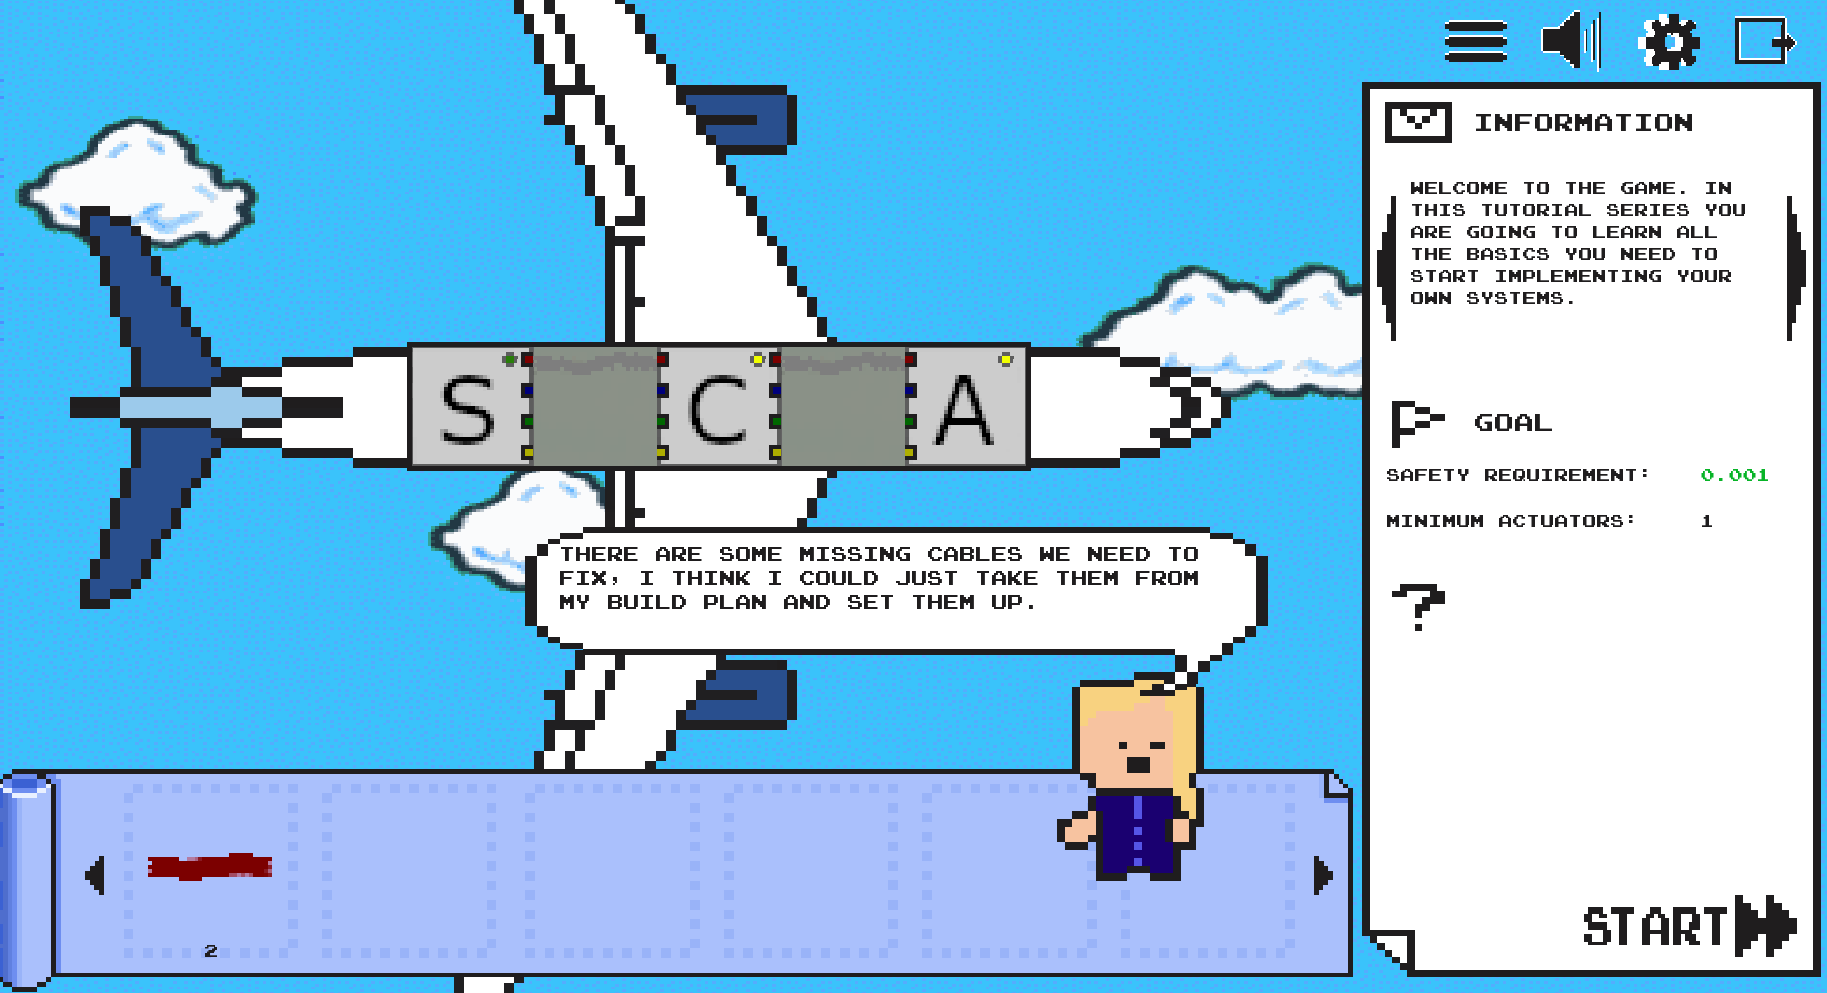
\includegraphics[width=\textwidth]{Pictures/res/implementation/scenes/tutorial-game-scene}
    \caption{Tutorial Scene with dialogue to explain basic gameplay}
    \label{fig:basic-gameplay-tutorial}
\end{figure}
\begin{figure}
    \centering
    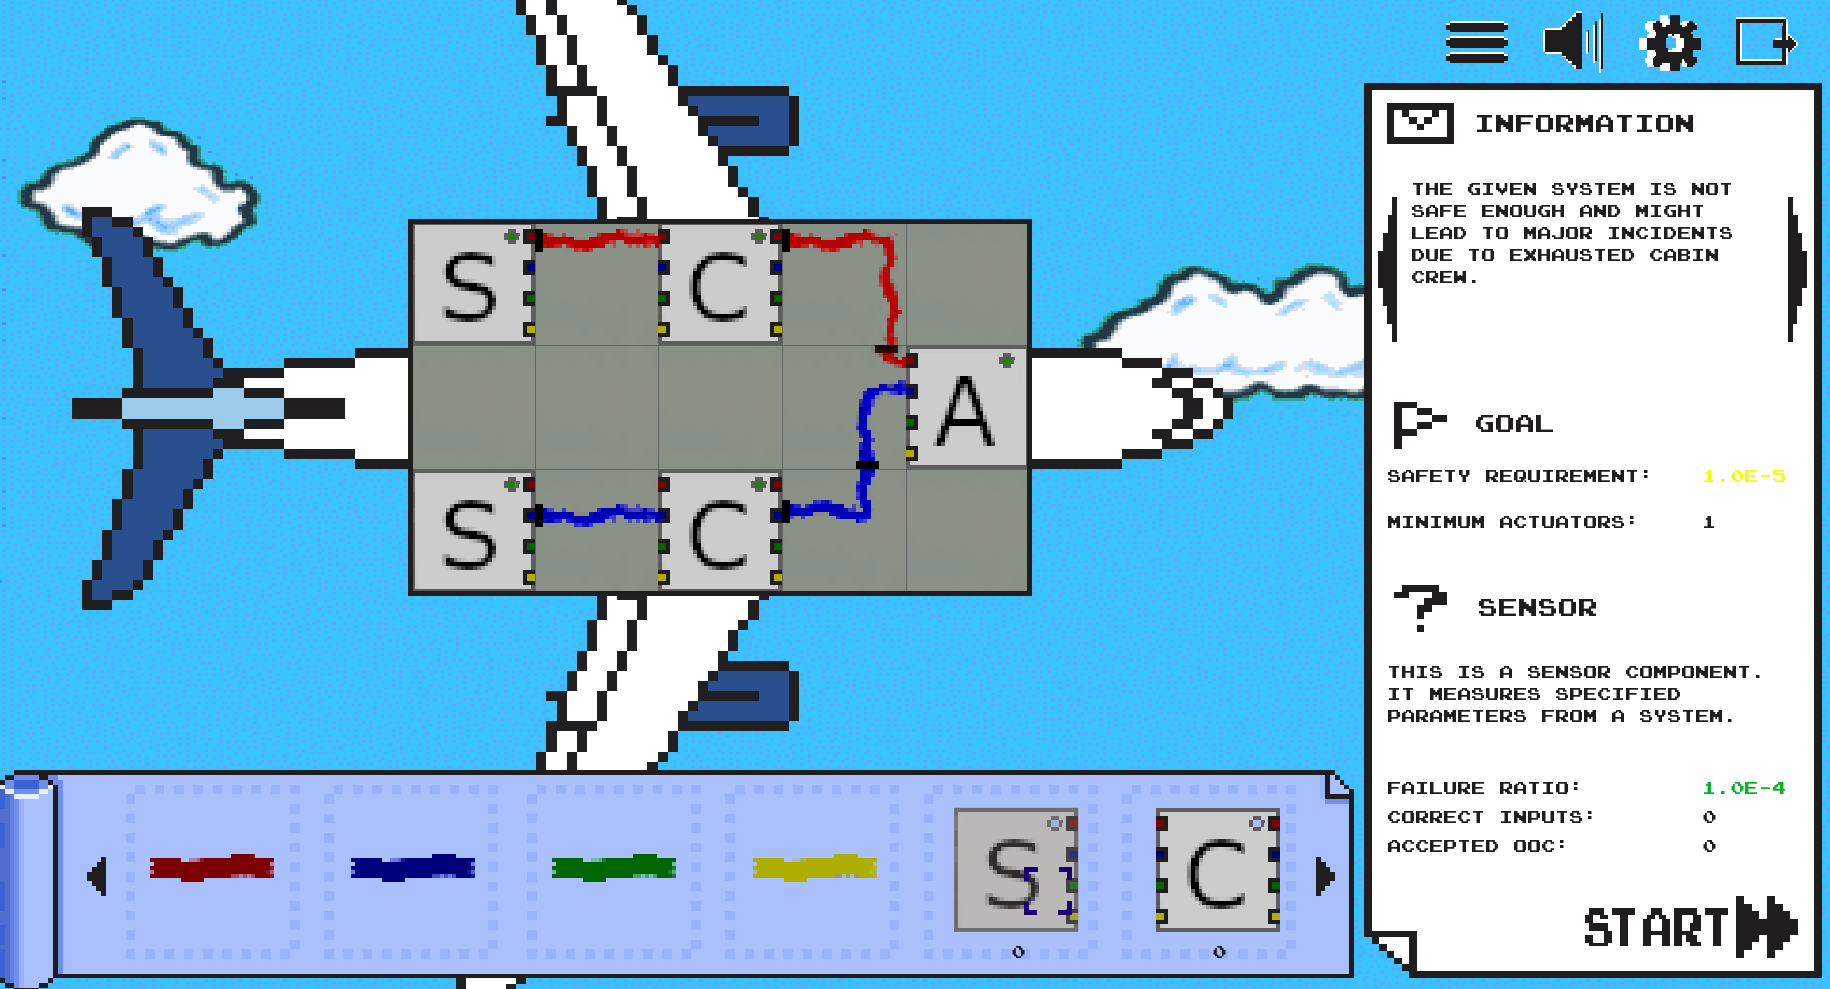
\includegraphics[width=\textwidth]{Pictures/res/implementation/scenes/duplex-scene}
    \caption{Scenario to set up a duplex system}
    \label{fig:duplex-system}
\end{figure}
\begin{figure}
    \centering
    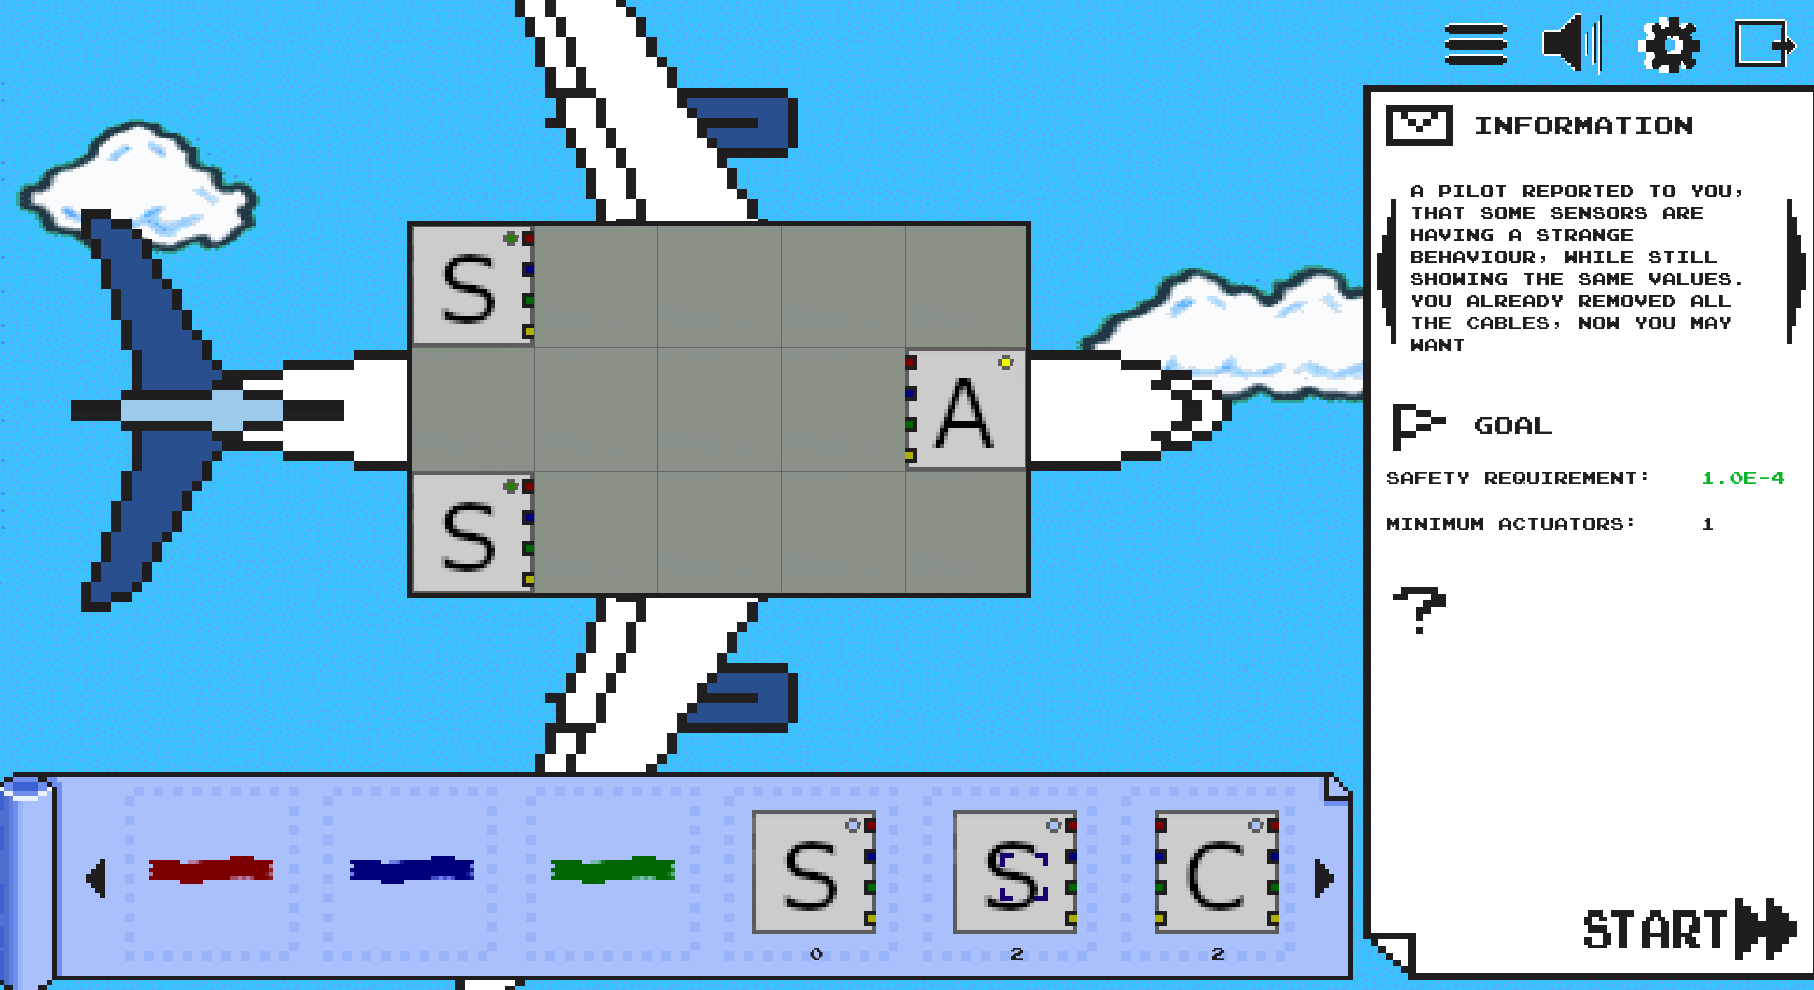
\includegraphics[width=\textwidth]{Pictures/res/implementation/scenes/cmf}
    \caption{Multiple useable sensors to visualize common mode failures}
    \label{fig:common-mode-scene}
\end{figure}
\begin{figure}
    \centering
    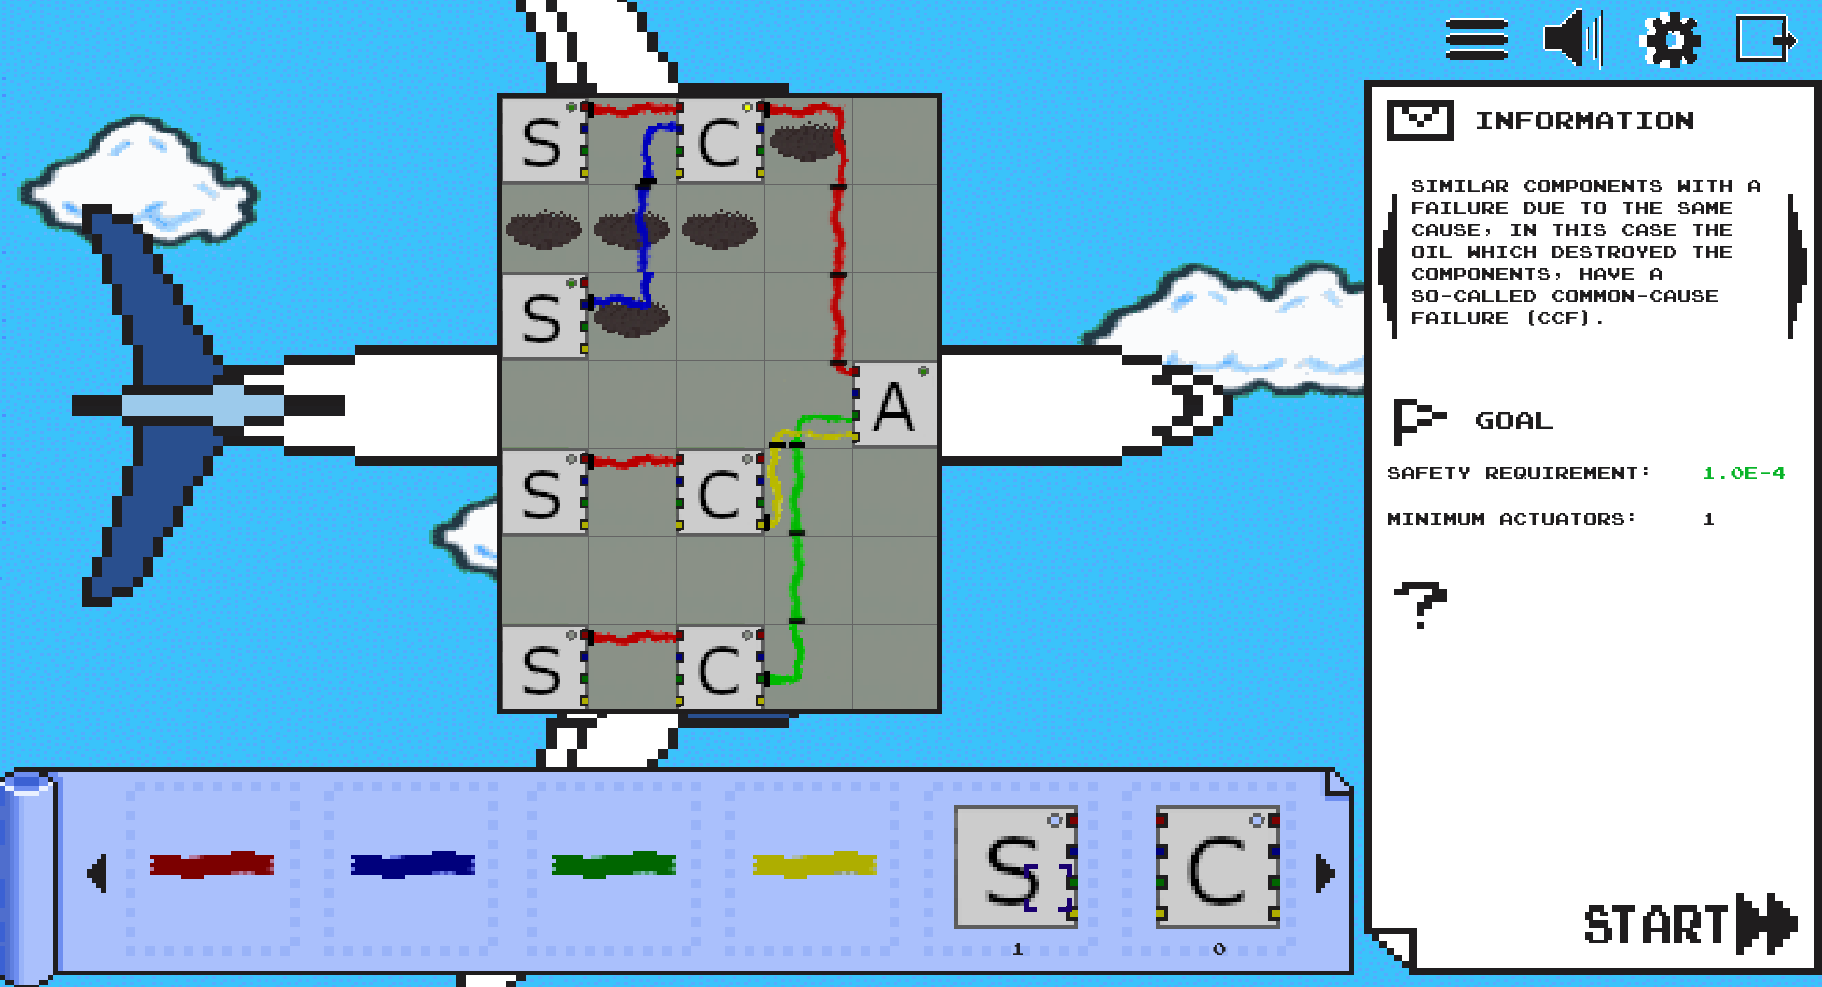
\includegraphics[width=\textwidth]{Pictures/res/implementation/scenes/oil-leak}
    \caption{A scene with an oil leakage on one side of the system to visualize common cause failures}
    \label{fig:common-cause-scene}
\end{figure}

For the game grid, tile sets as explained in section~\ref{subsec:tileset} are used, which consist of different seamless images for each of the
components, backgrounds and placeholders.
Figure~\ref{fig:tileset} shows all tiles that are currently available to the game implementation.
This is easily extendable by adding more tiles to the set, which may be used for backgrounds, placeholders or new simulation entities.
\begin{figure}
    \centering
    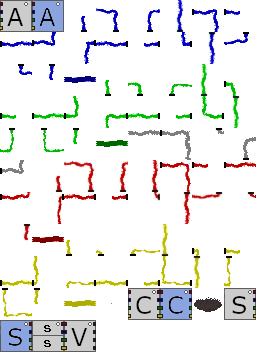
\includegraphics[width=\textwidth]{Pictures/res/implementation/tileset}
    \caption{Tileset}
    \label{fig:tileset}
\end{figure}

\subsubsection{Tutorial Scenes}\label{subsubsec:tutorial-scenes}
To elucidate the gameplay, tutorial dialogues have been incorporated into select scenes of the game.
To ensure that these dialogues are captivating and engaging, characters were crafted to make the tutorials more interactive.
The character models employed in the implementation can be seen in figure~\ref{fig:character-models}.
This framework is easily expandable, allowing for the addition of more characters to develop further tutorials,
dialogues, or even a storyline in the future, utilizing these character designs.
\begin{figure}
    \centering
    
\includegraphics[width=\textwidth]{Pictures/res/implementation/character-models}
    \caption{Character Models (left to right): Tina Technician, Ingo Engineer, Pete Pilot}
    \label{fig:character-models}
\end{figure}

\section{Data Storage \& Data Parsing}\label{sec:data-storage-&-data-parsing}
It was chosen to save and load resources from XML files, due to the benefits of this file format.
XML means \textit{eXtensible Markup Language}, and is a markup language that is used for encoding documents in a format that is easily readable for both human and computers.
It was designed to be flexible and extensible, allowing developers to create their own markup tags and structure data in a way that is specific to their needs~\cite{xml}.
\\
XML documents are made up of elements, which are enclosed in opening and closing tags, and attributes, which provide additional information about the element.
The structure of an XML document is defined by a \textit{Document Type Definition (DTD)} or an \textit{XML Schema}, which specifies the elements and attributes that are allowed in the document and the relationships between them.
\\
One of the main benefits of XML is its ability to store and transfer data in a standardized format that can be easily parsed by different software applications, regardless of the platform, and there are
already multiple implementations available to successfully do this, including JAVA's built-in library for DOM parsing~\cite{dom-parser}.
\\
The structure of the different XML files for levels, tilesets, scores and language used in this project will be explained in the next chapters.
\subsection{Tileset}\label{subsec:tileset}
A tileset file contains a list of multiple tile nodes, which each have an id and a type attribute.
A tile always contains exactly one image node, which has at least width, height and a resource path to an image assigned to it.
Optionally, there can also be a description attribute which can be used to set a tooltip that will be rendered to the games tooltip panel, if available.
\\
The code snippet shown in figure~\ref{fig:xml-tileset} shows a tileset with a single tile of the type Computer, including its description and image parameters.
\\ \\
\begin{figure}
\begin{lstlisting}[language=XML,label={lst:tileset-xml}]
    <?xml version="1.0" encoding="UTF-8"?>
    <tileset name="tiles">
        <tile id="200" type="COMPUTER">
            <image width="32" height="32" source="res/avionics/default.png" description="Default CPU Component"/>
        </tile>
    </tileset>
\end{lstlisting}
    \caption{XML Schema of the tileset file}
    \label{fig:xml-tileset}
\end{figure}
\subsection{Level Files}\label{subsec:level-files}
The root node of a level structure is the map node, which always includes attributes for assigning an id, a name,
a difficulty level (tutorial, easy, medium, hard, or custom), and grid dimensions (width and height) for the game grid.
The map node consists of a subnode for descriptions (and description parts, if the text should be divided into multiple displayable segments),
a subnode for available building elements from the build panel, and a subnode defining the pre-existing objects on the grid.
\\
Moreover, the goal and goal definition subnodes provide information on the criteria for completing a level (e.g.,
safety requirements, minimum components that must function correctly, and maximum out-of-control components).
The tileset used by the map must be specified in the tileset subnode,
and level unlocks (e.g., which level ids become accessible after completing the current level) can also be defined.
\\
The code snippet shown in figure~\ref{fig:xml-level} demonstrates an example of the level XML file structure, which depicts a 5x3 game grid with one actuator at position $x = 4$ and $y = 1$,
and two sensors at positions $x = 0$ and $y = [0, 2]$.
\\
It is important to note that the width and height attributes represent the actual map size, similar to the length of an array in Java,
while the positions indicate the grid positions starting at 0, akin to indexes in Java arrays.
\begin{figure}
\begin{lstlisting}[language=XML,label={lst:level-xml}]
    <?xml version="1.0" encoding="UTF-8"?>
    <map id="0" name="@0" width="5" height="3" difficulty="EASY">
        <description>
            <part>@1</part>
        </description>
        <goal>1e-7</goal>
        <goalDefinition workingActuators="1" workingSensors="0" workingComputers="0"/>
        <tileset source="base_tiles.xml"/>
        <unlocks>
            <unlock>6</unlock>
        </unlocks>
        <build>
            <entity id="500" amount="1000" safety="0" correctSignalsNeeded="1" outOfControlSignalsAccepted="0"/>
            <entity id="501" amount="1000" safety="0" correctSignalsNeeded="1" outOfControlSignalsAccepted="0"/>
            <entity id="502" amount="1000" safety="0" correctSignalsNeeded="1" outOfControlSignalsAccepted="0"/>
            <entity id="203" amount="2" safety="0" failureDetectionRatio="1" correctSignalsNeeded="1"
                    outOfControlSignalsAccepted="0"/>
        </build>
        <layer id="0" name="Tile Layer 1">
            <entity x="0" y="0" id="201" interactable="false" safety="1e-4" failureDetectionRatio="1"
                    correctSignalsNeeded="0" outOfControlSignalsAccepted="0"/>
            <entity x="0" y="2" id="201" interactable="false" safety="1e-4" failureDetectionRatio="1"
                    correctSignalsNeeded="0" outOfControlSignalsAccepted="0"/>
            <entity x="4" y="1" id="205" interactable="false" safety="0" failureDetectionRatio="1" correctSignalsNeeded="2"
                    outOfControlSignalsAccepted="0"/>
        </layer>
    </map>
\end{lstlisting}
    \caption{XML Schema of a level file}
    \label{fig:xml-level}
\end{figure}
\subsection{Language Files}\label{subsec:language-files}
A language file, as displayed in figure~\ref{fig:xml-lang} contains all text content used in the game for a specified language.
In the root node, the language type can be given according to the IETF language tag \todo{add source}, if supported by the game (i.e.\ implemented in the language manager).
Within this root node, string nodes are created which contain the id of a string as an attribute and the actual content as text.
Each of the ids has to be unique, otherwise only the first specified id will be considered in the implementation.
\\
\begin{figure}
\begin{lstlisting}[language=XML,label={lst:lang-xml}]
    <strings language="DE_DE">
        <string id="1">Sample Text</string>
    </strings>
\end{lstlisting}
    \caption{XML Schema of a language file}
    \label{fig:xml-lang}
\end{figure}

\subsection{Score Files}\label{subsec:score-files}
Highscores for each level are saved in a separate xml file containing information about the profile name, score and level id.
The schema shown in figure~\ref{fig:xml-score} is used for this file, saving the score 91 for a user who played level id one.
\\
\begin{figure}
\begin{lstlisting}[language=XML,label={lst:score-xml}]
    <scores>
      <scoreItem>
        <name>User</name>
        <score>91</score>
        <level>1</level>
      </scoreItem>
    </scores>
\end{lstlisting}
    \caption{XML schema of a score file}
    \label{fig:xml-score}
\end{figure}

\subsection{Parsing}\label{subsec:parsing}
For data parsing, a standard DOM parser library provided by Java is used.
It handles all possible exception types, such as input exceptions or malformed xml documents by default, which are added to the log of the game
and allows for a quick setup of parsing
the necessary nodes, attributes and text contents from the given input files.
As each type of file handled by default for this game has a different structure, the ResourceManager and its sub managers implement methods to handle
each file structure: loading a level, loading a tileset, loading scores, loading language data and loading fonts.

\section{External Device Inputs}\label{sec:external-device-inputs}
Since the game developed within the scope of this project is primarily intended for a younger audience at public events,
it was essential to accommodate not just mouse and keyboard inputs, but also gamepads.
This is because gamepads contribute to a more game-like atmosphere for users, while avoiding possible wrong inputs made by
other peripherals that can not be processed by the game.
This chapter will discuss the integration of gamepads, including game controllers, into the game.
\subsection{Mouse \& Keyboard}\label{subsec:mouse-&-keyboard}
The standard input device for the game are mouse and keyboard.
\subsection{Gamepad Integration}\label{subsec:gamepad-integration}
For gamepad integration, the open source library \textit{Jamepad} is used.
It automatically detects most USB controller devices and has an inbuilt button mapping which can be used in the implementation.
A separate thread captures game pad inputs, as actions may occur in between the calculated frames of the game engine.
Button handling is implemented in a way that a button press creates a new mouse event and the cursor position which is then handled by the action
systems' mouse event handling method.
This reduces maintenance and new implementation of buttons and actions, while being guaranteed to work correctly with all devices.
The game may also be played without a gamepad, however it is recommended to use the gamepad at least during public events.